%\documentclass[preprint]{aastex}  % USE THIS TO MAKE BIB, THEN FORMAT USING 
%EMULATEAPJ
\documentclass[twocolumn,numberedappendix]{emulateapj} \shorttitle{PSA64}
\shortauthors{Ali, et al.}

\usepackage{amsmath} \usepackage{graphicx} \usepackage[figuresright]{rotating}
%\usepackage{rotating}
\usepackage{natbib}
%\usepackage{pdflscape} \usepackage{lscape}
\citestyle{aa}

\def\b{\mathbf{b}} \def\k{\mathbf{k}} \def\r{\mathbf{r}} \def\q{\mathbf{q}}
\def\b{\mathbf{b}} \def\kp{\mathbf{k}^\prime}
\def\kpp{\mathbf{k}^{\prime\prime}} \def\V{\mathbb{V}} \def\expval#1{\langle #1
\rangle} \def\At{\tilde{A}} \def\Vt{\tilde{V}} \def\Tt{\tilde{T}}
\def\tb{\langle T_b\rangle} \newcommand{\vis}{\mathbf{v}}
\newcommand{\x}{\mathbf{x}} \newcommand{\xhat}{\hat{\mathbf{x}}}
\newcommand{\A}{\mathbf{A}} \newcommand{\N}{\mathbf{N}}
\newcommand{\C}{\mathbf{C}} \newcommand{\Q}{\mathbf{Q}}
\newcommand{\rhat}{\hat{\mathbf{r}}}

\begin{document} \title{PSA-64 Power Spectrum}

\author{ Zaki S. Ali\altaffilmark{1}, Aaron R. Parsons\altaffilmark{1,2}, Jeff
Zheng, Jonathan C. Pober\altaffilmark{4}, James E. Aguirre\altaffilmark{3},
David R. DeBoer\altaffilmark{2}, Daniel C. Jacobs\altaffilmark{8}, Adrian
Liu\altaffilmark{1}, David F. Moore\altaffilmark{3}
% XXX if includes paper data, needs full author list
}
%\tableofcontents

\altaffiltext{1}{Astronomy Dept., U. California, Berkeley, CA}
\altaffiltext{2}{Radio Astronomy Lab., U. California, Berkeley, CA}
\altaffiltext{3}{Dept. of Physics and Astronomy, U. Pennsylvania, Philadelphia,
PA} \altaffiltext{4}{Physics Dept.  U. Washington, Seattle, WA}
\altaffiltext{8}{School of Earth and Space Exploration, Arizona State U., Tempe,
AZ}

\begin{abstract} \end{abstract}

% XXX fringe weighting profile XXX delay spectrum not violated by freq-dependent
% fringe rate weights

\section{Introduction} The hyperfine transition in the ground state of hydrogen
leads to the emission of the infamous 21 cm wavelength photon. The 21 cm
transition is thought to be one the most promising probes of the early universe
due to the fact that the frequency of observed radiation maps to a specific
redshift. It has the potential to map the never before seen dark ages
($z\sim{30}$), where the first galaxies and stars were beginning to form, as
well as when the Epoch of Reionization (EoR), when neutral hydrogen was
completely ionized by the photons emitted by the first sources. The wealth of
information that can be obtained from the use of this optically thin transition
include the formation of the first stars and galaxies, neutrino masses, and
initial inflation power spectrum, amongst other science (list and cite
exhaustively). Using 21 cm to map the universe has the ability to surpass the
Cosmic Microwave Background (CMB) in terms of the wealth of science it can
deliver. Refer to \cite{furlanetto_et_al2006}, \cite{morales_wyithe2010}, and
\cite{pritchard_loeb2012} for reviews on using the 21 cm transition as a
cosmological probe.

There are two different approaches to probe the 21 cm transition - via
statistical power spectrum measurements or by measuring the \emph{global} 21 cm
signal, which is the mean of the signal over the entire sky. Both of these
techniques have their merits and many experiments are aimed to detect neutral
hydrogen during EoR and the dark ages. GMRT (\cite{paciga_et_al2011}),
LOFAR(\cite{rottgering_et_al2006}), MWA(\cite{tingay_et_al2013}),
PAPER(\cite{parsons_et_al2010}), and 21CMA are all aiming for the power spectrum
detection of the fluctuations in the 21 cm line, whereas experiments like EDGES
(\cite{bowman_et_al2010}), LWA, LEDA (\cite{lincoln_bernardi_2012}), DARE
(\cite{burns_et_al2012}) , and SciHi (\cite{tabitha_et_al2014}) are after the
mean brightness temperature of 21 cm relative to the CMB background. 

Like CMB experiments, foreground contamination is a major concern for 21 cm
experiments. Sources of foregrounds for these low frequency experiments include
synchrotron radiation from the Milky Way, extragalactic radio sources and
supernova remanants. Since all 21 cm experiments are low frequency by nature
(ranging from 50MHz - 200MHz), emission from these foregrounds drastically
drowns out the faint EoR signal by atleast 5 orders of magnitude
(\cite{furlanetto_et_al2006}, \cite{santos_et_al2005}) at these frequencies; the
sky is much brighter at low frequencies than higher frequencies owning the the
power law spectral distrbutions of sources. However, because the brightest
foregrounds are spectrally smoothe, many techniques have been developed to use
this fact to isolate and remove foregrounds (\cite{morales_et_al2006a},
\cite{bowman_et_al2009}, \cite{liu_et_al2009}, \cite{liu_tegmark2011},
\cite{parsons_et_al2012b},\cite{dillon_et_al2013a}).

Currently, the best statistical upper limit on the 21 cm power spectrum was made
with PAPER and is held at $(41 mk)^{2}$ at $k=.27 h \text{Mpc}^{-1}$. However,
all major 21 cm experiments (LOFAR, MWA, and PAPER) are at the cusp of detection
and all have the sensitivity to rule out the optimistic reionization scenarios.
However, even with a detection from anyone of these experiments, the
characterization of the 21 cm power spectrum and imaging of EoR will have to
wait until future 21 cm experiments such as the Hydrogen Epoch of Reionization
Array (HERA) and the Square Kilometer Array (SKA) which will have more raw
collecting area and greater sensitivity. 

In addition to using the 21 cm transtion as a probe of the early universe, many
other techniques have been used to constrain reionization parameters such as
the redshift of reionization (when the neutral fraction, $\bar{x} = 0.5$), the
duration of reionization, and the end of reionization, amogst others. The
Gunn-Peterson effect has shown that the intergalactic medium was fully ionized
by $z=6$ (\cite{fan_et_al2006}). The most recent results from SPT have shown
the constraints of the duration of reionization to be  $\Delta{z} \textless 5.4$
(\cite{george_et_al2014}) using results from the kinetic Sunyaev-Zel'dovich
effect. The optical depth parameter, $\tau$, from the CMB also constrains
reionization with the Panck results (\cite{planck_et_al2013}) and CMB
polarization (\cite{page_et_al2007}). Lyman emitters and lyman alpha absorption
profiles towards distant quasars have also given limits on the end of
reionization
(\cite{schenker_et_al2013,treu_et_al2013,faisst_et_al2014,bolton_et_al2011}.

This paper reports on the results from the Donald C. Backer Array for Probing
the Epoch of Reionization (PAPER) -  64 antenna dual polarization minimum
redundancy configuration.  The paper is outlined as follows. In section
\ref{sec:observations} we describe the observations used in this analysis. In
\ref{sec:improvements} we discuss the improvements in this pipeline with respect
to the previous analysis of PSA-32 \cite{parsons_et_al2014a}. We then move on to
the data analysis pipeline in section \ref{sec:analysis}. Seciton
\ref{sec:results} describes the results of our efforts and provides new
contraints on EoR. We conclude in \ref{sec:conclusion}.

\begin{figure*}[!t]\centering
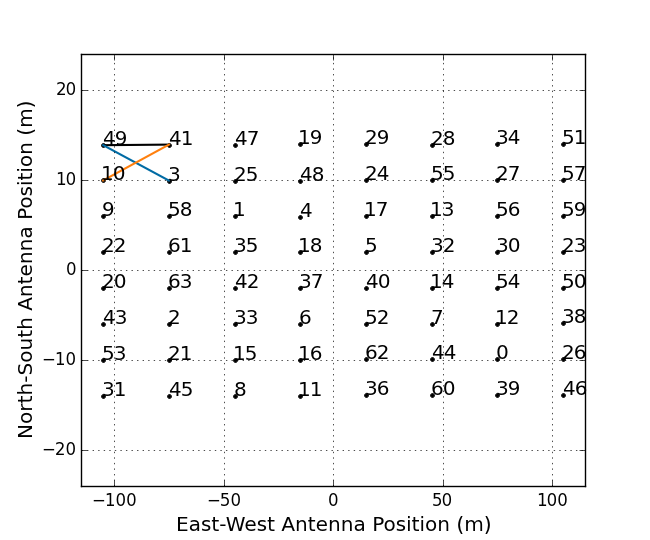
\includegraphics[width=1.85\columnwidth,height=\columnwidth]{plots/antenna_positions.png}
\caption{Antenna positions for the PAPER 64 observation run.}
\label{fig:antenna_positions}
\end{figure*}



%%%%%%%%%%%%%%%%%%%%%%%%%%%%%%%%%%%%%%%%%%%%%%%%%%%%%%%%%%%%%%%%%%%%%%%%%%%%%%%%%%
\section{Observations}\label{sec:observations}
PAPER is a driftscan array deployed at the Square Kilometer Array South Africa
(SKA-SA) reseve in the Karoo desert located at (21:25:41:9,
-30:43:17:15)(\cite{parsons_et_al2010}) . Observations discussed in this paper
were taken while PAPER consisted of 64 dual polarization antennas deployed in
the Fall of 2012. The array was configured into a maximally redundant antenna
layout (see figure \ref{fig:antenna_positions}) where multiple baselines measure
the same fourier mode on the sky
(\cite{parsons_et_al_2012},\cite{parsons_et_al2014a}). The PAPER antennas are a
cross-dipole design in which both polarizations (X and Y) are processed
independently. The PAPER beam is speactrally and spatially smooth down to the
horizon with a $60^{\circ}$ FWHM (\cite{jacobs_et_al2011},
\cite{parsons_et_al2010}, \cite{stefan_et_al2013}). 

The PAPER-64 correlator processes a 100 MHz to 200 MHz bandwidth, first
channelizing the 100 MHz band into 1024 channls of width 97.6 kHz, and then
cross multiplying every antenna and polarization with one another for a total of
8256 cross products, including auto correlations. The architecture of this
correlator is based on CASPER open source, reconfigurable hardware
(\cite{parsons_et_al2008}). The channelizer, which includes the PFB-FFT and
corner turn, consisted of 16 ROACH boards with eight 8 bit analog to digital
converters. The cross multilication engine (X engine) was moved to GPU's based
on the X-GPU, a general purpose X engine for GPU's (mike clark xgpu 2011?). 
Visibility cross products are integrated for 10.7 seconds on the GPU's before
being written to disk. We write all stokes parameters to disk, however the
analaysis described here only apply to the XX and YY polariztion products.

We rely on all 2016 (for each polariztion) baselines for the calibration
procedure, but only use a subset of the baselines for the power spectrum
analysis. This subset encompases 3 separation types; the shortest spaceing
east-west baselines (e.g. 41-47) and those of the same East-West column spacing,
except slanted up and down one row (e.g. 10-41 and 10-58, respectively).
Baselines in each of the 3 separation types (or redundant groups) are
instantaneously redundant within the group and therefore measure the same
fourier modes on the sky. This allows us to coherently add fourier modes,
building sensitivity as $N$  rather than $\sqrt{N}$.

The observation of this 64 antenna data set spanned a 135 day period that
commenced on 2012 November 8 (JD62456240) and ended  2013 March 23 (JD62456375). 
For the power spectrum analysis, we use data that spanned, in local sidereal
time (LST), a range of 0:00 to 10:00 hours. This range corresponds to
the "EoR cold patch", in which galactic synchrotron power is minimal (away from
the center of the galaxy). Due to LST drift of 3:56 minutes every solar ay, we
unevenly sample every lst in our observations, giving us more samples of certain
lsts than others. The lsts with the greatest number of smaples are those used in
the power spectrum analysis (along with those corresponding to the cold patch).
Figure \ref{fig:coverage} shows our observing field with the contours labeling
the beam weighted observing time relative to the peak, directly over head the
array.
%XXX lst range will change.

\begin{figure*}[!t]\centering
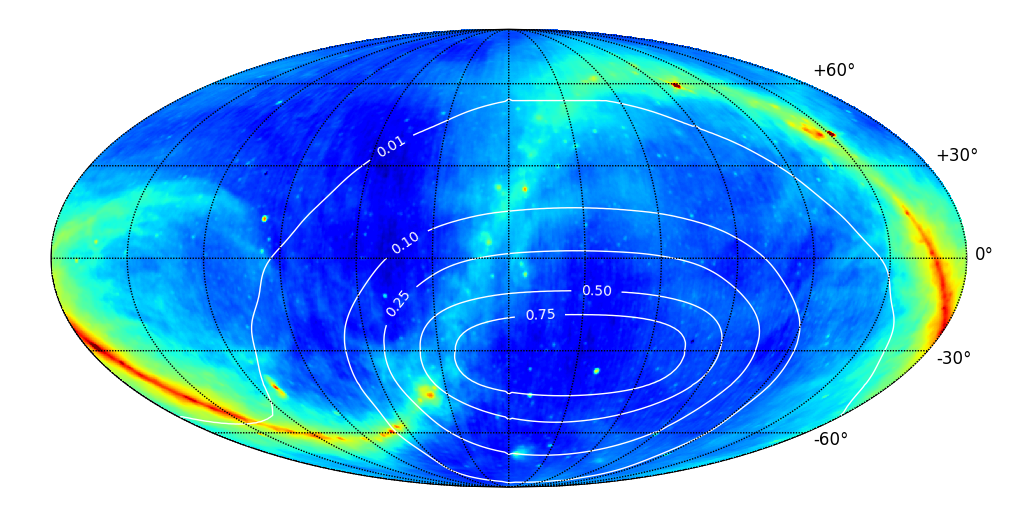
\includegraphics[width=2\columnwidth,height=\columnwidth]{plots/coverage.png}
\caption{The PAPER field. Contours are the beam weighted observing times
relative to the peak observing time/beam.}
\label{fig:coverage}
\end{figure*}



\section{Analysis}\label{sec:analysis}
XXX FLOW CHART FIGURE XXX
We now describe the analysis pipeline leading up to the final power spectrum
measurement of our data set. To begin, we run a compression algorithm to reduce
the data volume of our raw data. This step, described in the appendix of
\cite{parsons_et_al2014a}, reduces data volume by a factor of 40. We then
calibrate on the basis of redundancy before using self-calibration
to solve for the absolute phase and gain parameters. After suppressing
foregrounds with a wide-band delay filter, we average the data in local
sidereal time and apply a fringe rate filter to optimally combine the
time domain data. Finally, we use optimal quadratic estimators to make our
estimate of the 21 cm power spectrum.  Figure \ref{fig:analysis_pipeline} shows
a block diagram of the analysis pipeline and includes some information on
simuations and signal loss.

\section{Calibration}\label{sec:calibration}
The calibration procedure employed in this analysis is twofold: a relative
calibration and an absolution calibration. The relative calibration employed
uses the fact that PAPER contains numerous redundant baselines. As usual, the
absolute calibration uses the usual self calibration methods employed by radio
interferometers. Here we describe both procedures.

\subsection{Relative Calibration}
%    -Principles of redundant calibration. Fact that there is no signal loss in
%       this kind of measurement.
%       --PAPER has a redundant configuration. Therefore the number of baselines
%         is larger than the number of unique baselines in the array. There are
%         multiple baselines that measure the same sky.
%       --Introduce uniqe baseline. We define a unique baseline to be the set of
%         redundant baselines of a unique orientation.
%       --All baselines of a unique baseline measure the same sky and
%         therefore, differences between them are what need to be calibrated
%         out. These are the gain variations imparted on the incoming signal by
%         the antenna.
%       --There is no signal loss in this method. Sky signal is the same for
%         each of the redundant baselines is the same and hence any algorithm that
%         preserves common mode signal (which is what redcal does) is necessarily
%         lossless. This is an important point!  
%       --In addtion, because gains are normalized to have a unity magnitude the
%         input arn output flux scale are the same. (This is an omnical thing)
%         
%    -What can we solve for and what can't we solve for. We can solve for the
%     relative complex gains between antennas, but not the absolute gain and phase.
%       --Because redundant calibration does not fold in any outside
%         information about the sky that we are observing, it inherently is a
%         relative calibration scheme that solves for the relative gains and
%         phases of antennas within the array. 
%       --Therefore, we cannot solve for the absolute phase and gain of the
%         array. There is not enough information.
%       --Absoulte phase and gain calibration are addressed in later sections.
%

The highly redundant configuration of PAPER lends itself to
use the redunancy in baselines for a relative calibration between anteannas.
Multiple baselines of the same length and orientation measure the same sky
signal. On this basis, all of the differences between redundant baselines are
attributed to differences in the signal chain, including effects from variations
in antennas, cables lengths, and receivers. These are the variations that are
calibrated out and leads to relative calibration solutions between all the
antennas within the array.  Note that this relative calibration using redundancy
(i.e. redundat calibration) only constrains the relative complex gain solutions
between antennas and has no information about the sky. Furthermore, redundant
calibration inherently preserves common mode signal between redundant baselines,
and therefore this type of calibration is necessarily lossless. 


%    -Summary of the procedure of redundant calibration. This should be mixed in
%     with the equations from Zheng et. al.
%       --Two flavors of redundant calibration : logcal and lincal. Cite
%         liu,zheng.
%       --logcal takes log of equation 3 in zheng et. al., and thus becomes a
%         linear system. Can then solve for the log of the antenna gains, as
%         well as the true visibility of the sky as measured from a unique
%         baseline. 
%       --lincal is the linearization via taylor expansion of the same equation
%         3. This provides us with a better solution. The reason for doing
%         lincal is that logcal is a biased estimator. 
%       --Because there are more baselines than the number of unique baselines, 
%         we have an overdetermined system of equations and therefore can
%         uniquely solve for all of the gains and "true" visibilities.
Practiaclly, redundant calibration takes on two flavors, log calibration (logcal) and
linear calibration (lincal) (\cite{liu_et_al2010,zheng_et_al2014}). Logcal, takes
the logarithm of the visibility measured by an interferometer (equation 4 of
\cite{zheng_et_al2014}) to give a linearized system which can then be fit to
using linear least square. We are fitting to
\begin{equation}\label{eqn:logcal}
    \log{v_{ij}} = \log{g_{i}^{*}} + \log{g_{j}} + \log{y_{i-j}},
\end{equation}
where the $g_{i}$'s are the
complex gains of each antenna and $y_{i-j}$ is the visibility of the given
baseline if it measured the perfect sky. Redundancy gives us an overconstrained
system of equations and we can thus solve for complex gains from each antenna
using traditional linear algebra techniques.  In addition we also get a model
visibility of for a given given baseline.  Averaging these models together for
redundant baselines gives us a an estimate of our model visibility for a given
baseline type.

Lincal taylor expands the visibility around some initial estimates of the gains
and model visibilities via the equation 
\begin{equation}\label{eqn:lincal}
v_{ij} = g_{i}^{0*}g_{j}^{0}y_{i-j}^{0} + g_{i}^{1*}g_{j}^{0}y_{i-j}^{0} +
         g_{i}^{0*}g_{j}^{1}y_{i-j}^{0}+g_{i}^{0*}g_{j}^{0}y_{i-j}^{1},
\end{equation}
where the $0$ indexes are the intial estimates and the $1$ indexes are the
solutions we fit for. In the implementation, described below, the initial
estimates of the solutions are taken as the outputs of logcal. The benefit of
lincal is that it is not a biased estimator as opposed to logcal which takes the
logarithm of additive noise(\cite{liu_et_al2010}).

%    -How was this calibration applied to the data. 
%       --Using omnical package. Give credit jeff and url to omnical. Cite
%         paper.
%       --Implements both logcal and lincal. Discuss the speed ups. 
%       --gains were applied to the uv datasets and written out in the same
%         format. However, Omnical is quite general and solutions can be written
%         out in text files and adapted to other file formats.
%    
%    -Removing additive offset and what is the time cadence of all of this.
%       
%    -Diagnostic figures : Chi-squared, complex plane, stability vs. time and
%                          frequency.

Implementaion of redundant calibration was done with the ${Omnical}$ package, an
open source redundant calibration package written by Jeff Zheng
\footnote{https://github.com/jeffzhen/omnical}\cite{zheng_et_al2014}. This
package implements both logcal and lincal, solving for a complex gain solution
per antenna, frequency, and integration. The per integration solutions are then
applied to visibilities and the results are shown in \ref{fig:omniview}.

\begin{figure*}
\centering
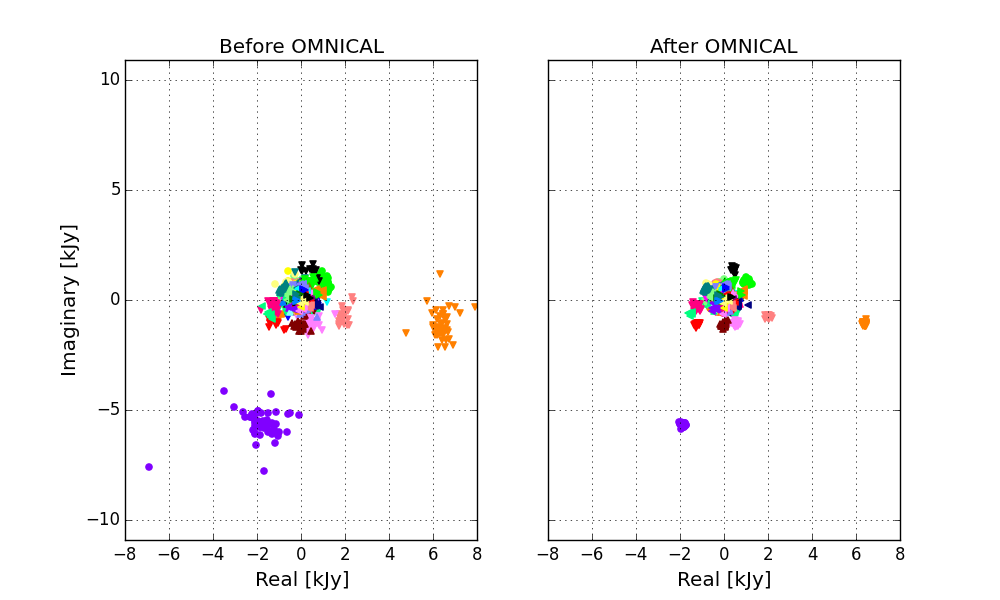
\includegraphics[width=2\columnwidth]{plots/omniview_64.png}
\caption{omniview plot.}
\label{fig:omniview}
\end{figure*}

\begin{figure}
\centering
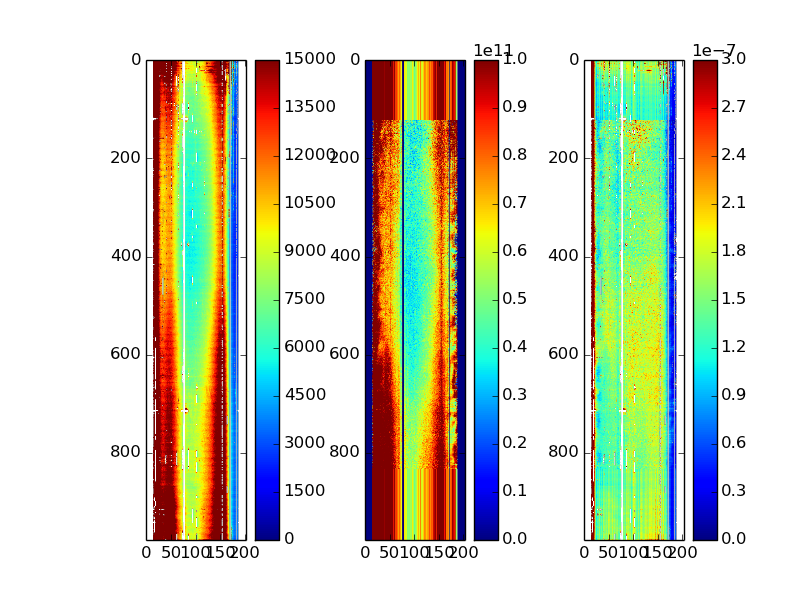
\includegraphics[width=\columnwidth]{plots/august_chi2.png}
\caption{chi squared}
\label{fig:chi2}
\end{figure}


In addition to solving for gain solutions, Omnical also characterizes the
quality of the calibration by calculating the $\chi^{2}$ for every integration.
Figure \ref{fig:chi2} shows the $\chi^{2}$ squared waterfall for a full
nights worth of calibrations. From \cite{zheng_et_al2014}, the
$\chi^{2}/\text{DoF}$, where $\text{DoF} = 2N_{baselines} - 2(N_{antennas} +
N_{\text{unique basleines}} $ is the number of degrees of freedom. For a good
fit, the $\chi^{2}/DoF$ is drawn from a mean 1 distribution with variance
$\frac{2}{\text{DoF}}$. The distribtuion of the $\xi^{2}$ in figure
\ref{fig:chi2} has a mean of 2, meaning that the fit was not the best to what
our noise model is.
The noise model used was obtained from the variance statistic calculated during
the binning of days in local sidereal time, which occurs after the
application of crosstalk removal, combining X and Y polarization, and the
wideband delay filter. Hence, the noise model may not be well suited for the
$\chi^{2}$, and is a likely reason that the distribution has a mean of 2.
%XXX This may change and we may get a chi-squared of around one.% 

The calibration parameters solved for in Omnical also have a time independent
additive offset associated with them, This additive offset is associated with
crosstalk between antennas, especially the shorter north south baselines.
To remove this crosstalk, Omnical calculates an averaged (over ten minutes)
additive offset that it subtracts from each visibility before running fitting
for solutions once again. This additive offset is in effect averaging deviations
from the $chi^{2}$ over 10 minutes and subtracting that deviation off.

\subsection{Absolute Calibration} 
%    -Selfcal to pictor, fornax, and crab (to get the north-south components).
%       --Reiterate that redundant cal does not solve for the overall flux and
%         phase parameters. 
%       --There are two final phase parameters we must solve
%         for in order to correctly phase to a source on the sky. Redundancy
%         only gets you so far, but still need to be able to unambiguously phase
%         to sources.
%       --We use self calibration to solve for the global phase parameters using
%         Pictor A, Fornax A, and Crab Nebula. 
%       --
%
%    -Diagnostic Plots: Show Field image from Bernardi. This will give
%     confidence in a good absolute phase calibration.

After solving for the relative complex gains of the antennas using redcal, an
overall phase and gain calibration needs to be solved for. We use the standard self
calibration (selfcal) method for radio interferometers to solve for the absolute
phase calibration. We used Pictor A, Fornax A, and Crab Nebula in our selfcal
fit for the overall phase solutions. Figure \ref{fig:field_image} shows an image
of the field with Pictor A (5:19:49.70, -45:46:45.0)  and Fornax A
(3:22:41.70,-37:12:30.0). The measured source positions are the same as the the
catalogue positions for these sources.

\begin{figure}[!t]
\centering
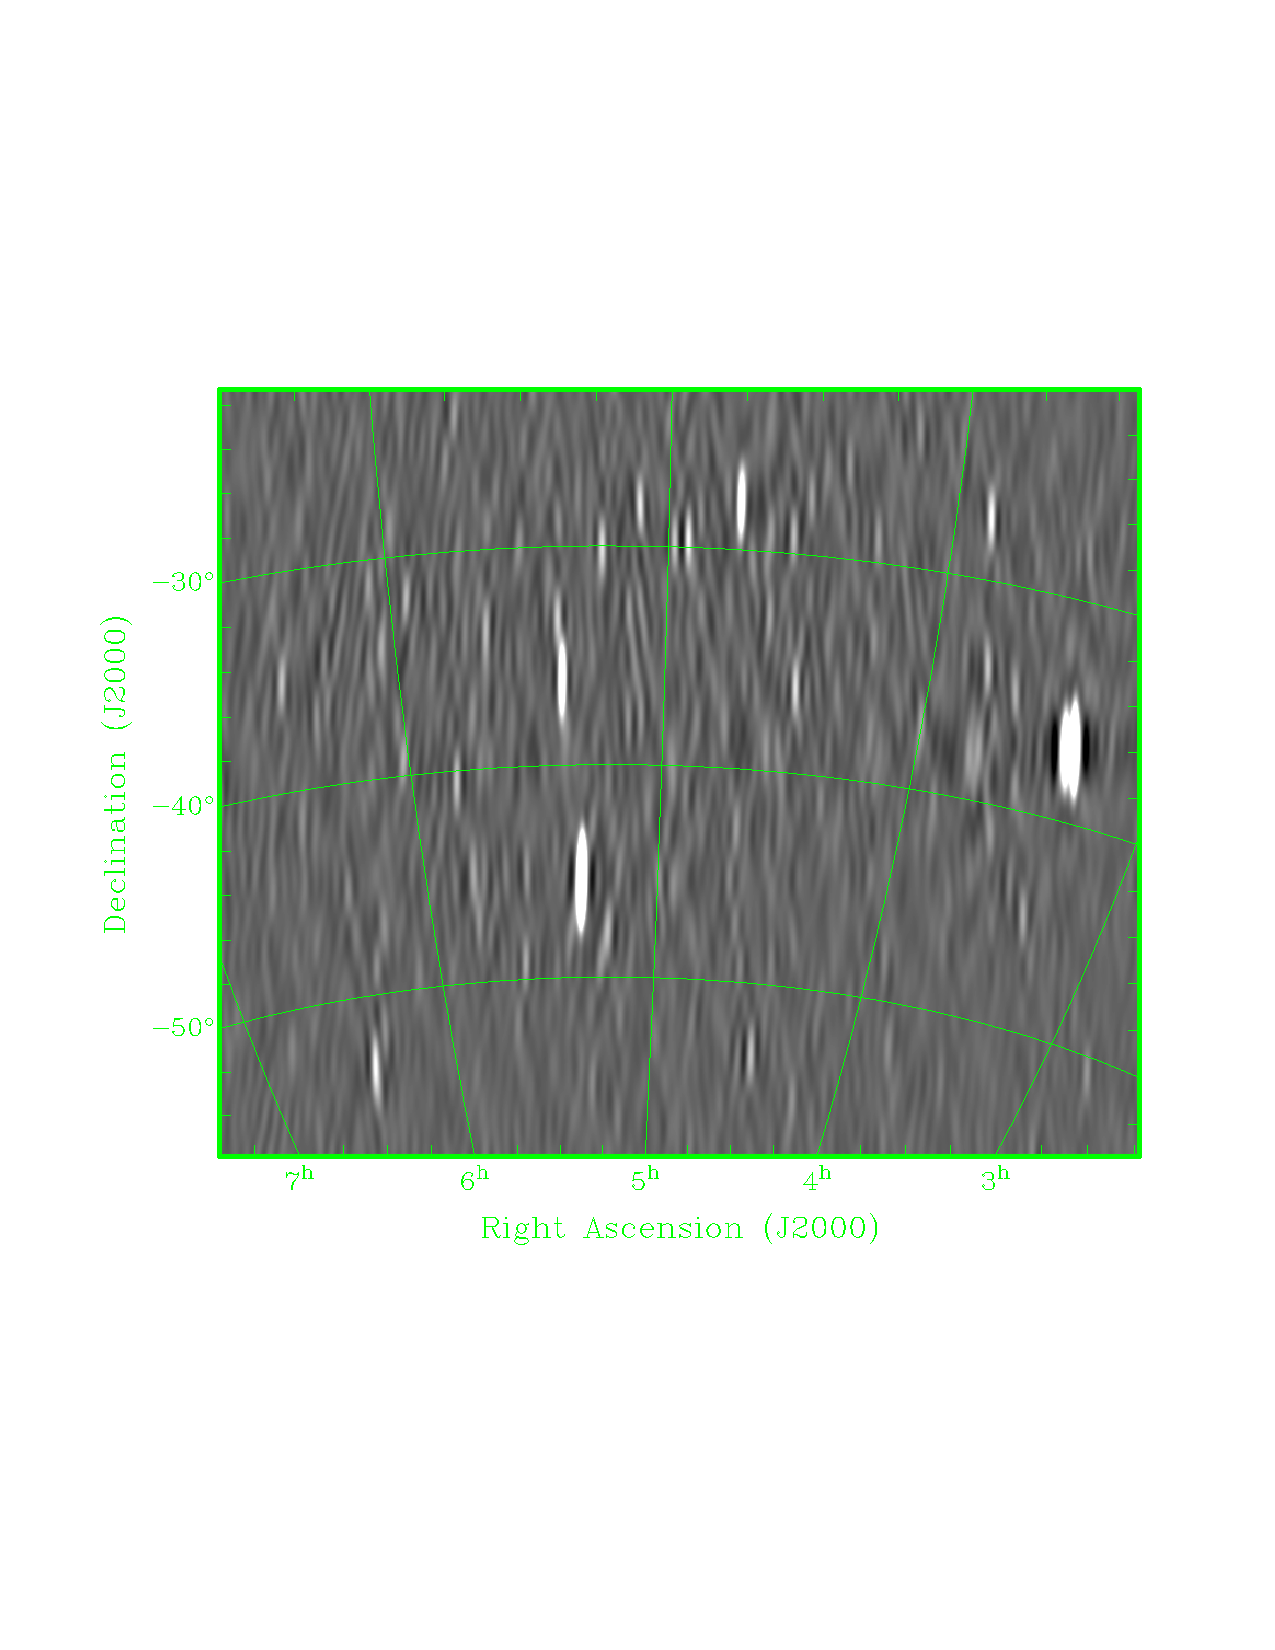
\includegraphics[width=\columnwidth]{plots/gianni_pic_image.pdf}
\caption{Image of Pictor.}
\label{fig:field_image}
\end{figure}


%    -Calibrated to Pictor A. 
%       --As before, redundant calibration cannot set a global flux scale. For
%       our measurements to be correct, we need to set a fluxscale. We use
%       Pictor A to set our fluxscale. Cite Dannys pictor paper.
%      
%    -Our bandpass model is a 9th degree polynomial. 
%       --In order to set our fluxscale, we beamform our data upto pictor A,
%         summing baselines, and then then fit a 9th degree polynomial to the
%         bandpass. This is our measure of the spectrum of Pictor A. 
%       --Because we are beamforming to pictor and fitting a polynomial to the
%         bandpass, there is signal loss. This signal loss is of the 
%    -Tabulate signal loss due to this model. Averaging over Nbls, times gives us
%     an average over independent uv modes.
%       --Working on this... a few questions about it.
%
%    -The actual signal loss on a given mode is L/N where L is the loss for a
%     single instance of the beamform (one time, one baseline) and N is the
%     number of baseline and times that were summed.
%
%    -PLOTS: 
%        --A plot that is the phased to pictor beamform gain 
%          (or maybe just a single channel for all days.
%        --The measured and theoretical pictor spectrum 
%        --A comparison to the PSA32 Flux CAL.

We then set our over all flux scale by using Pictor A as our calibrator source
with source spectra as derived in \cite{jacobs_et_al2013}, 
\begin{equation}
    S_{\nu} = S_{150}\times\left(\frac{\nu}{150MHz}\right)^{\alpha},
\end{equation}
where $S_{150} = 382 \text{Jy} \pm 5.4$ and $\alpha = -.76 \pm .01$, with
1$\sigma$ error bars.


To derive the source spectrum from our measurements, we use lst averaged data (see
section \ref{sec:lstbin}) containing foregrounds for the hour before and after from
where Pictor A transits. We image, in 15 minute snapshots for this data set,
every frequency channel. The source spectra is derived per snapshot and we average
these together, weighting by the primary beam in the direction of Pic A to get
the measured spectrum of Pictor A. To fit our bandpass, we divide the model
spectrum with ourAmeasured spectrum and fit a ninth-order polynomial over a
frequency range from 120-170MHz. Figure \ref{fig:pic_spec} shows the derived
Pictor A spectrum and the model spectrum derived from \cite{jacobs_et_al2013}.

\begin{figure}[!t]
\centering
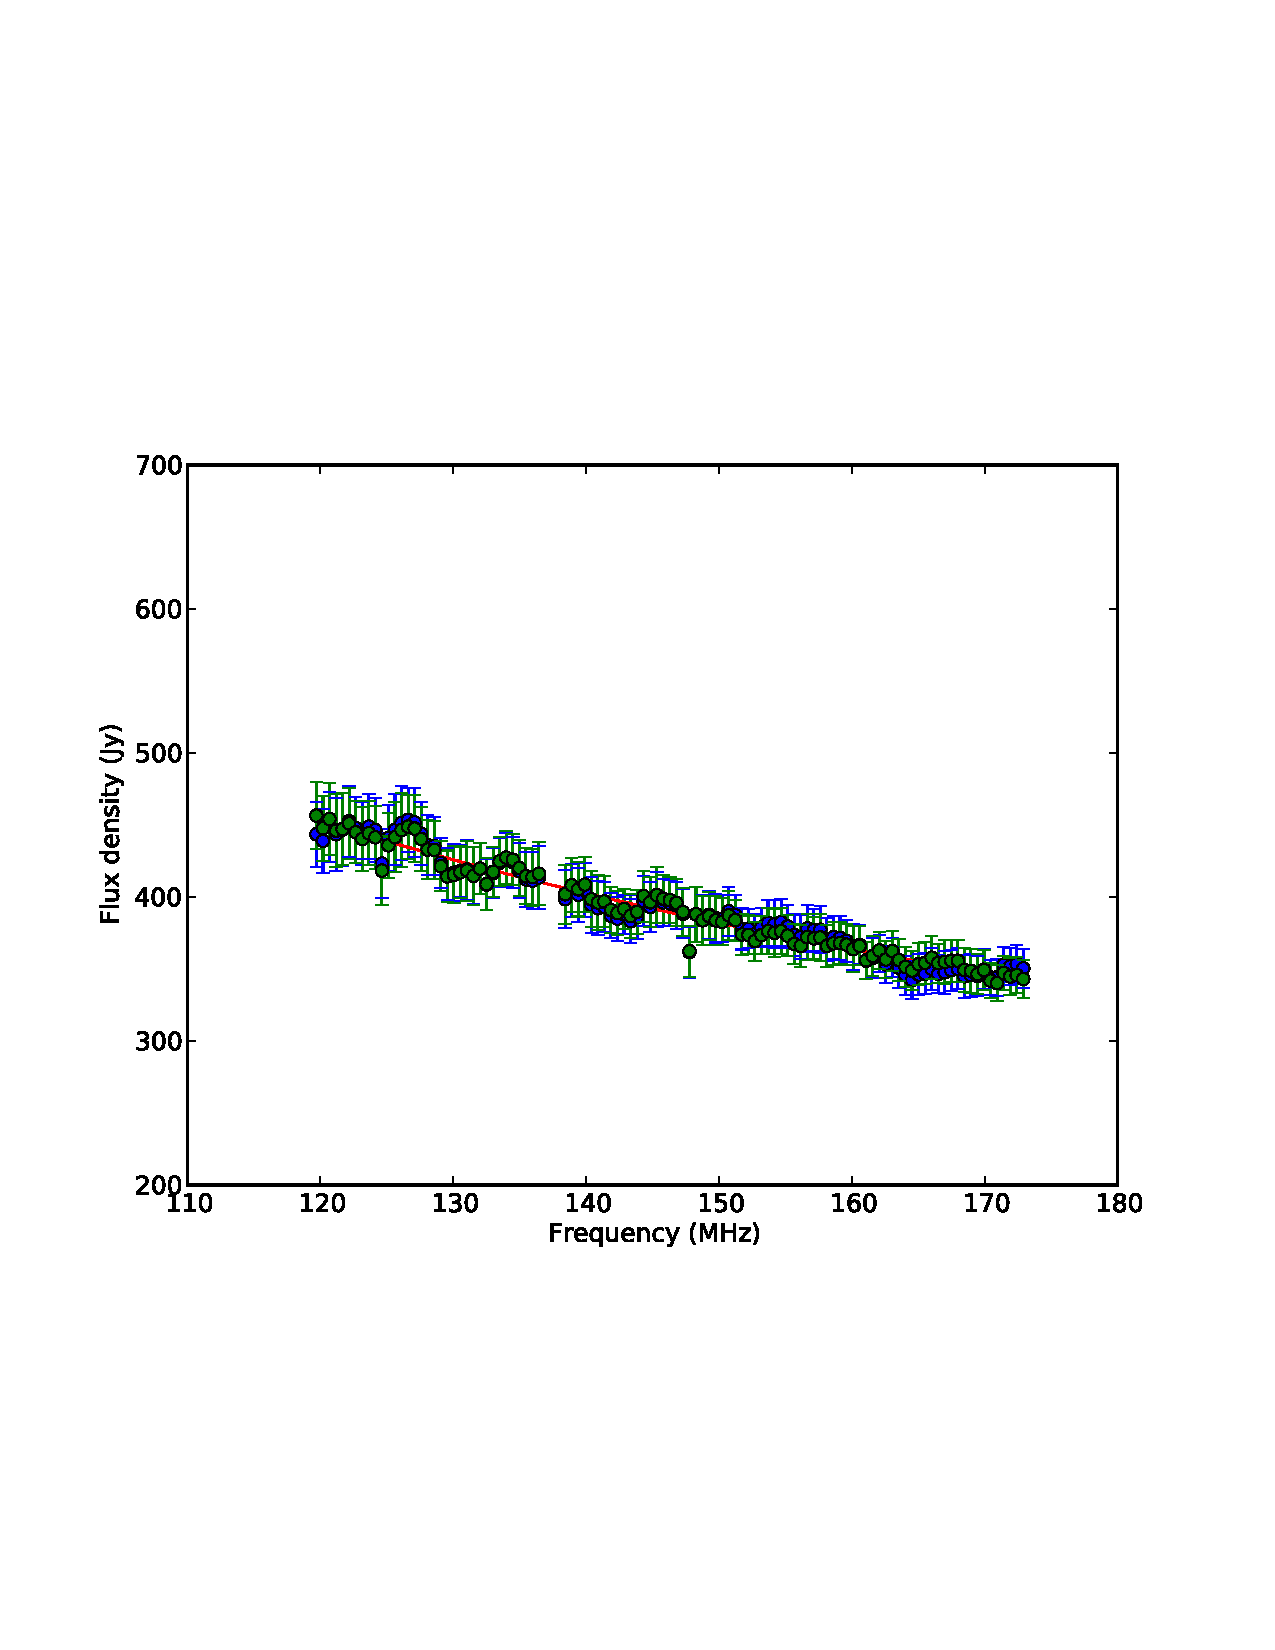
\includegraphics[width=\columnwidth]{plots/PicA_normalized_spectrum.pdf}
\caption{Pictor spectrum.}
\label{fig:pic_spec}
\end{figure}

Fitting a polynomial to the bandpass has the potential for signal loss which
would include fitting out some modes of the EoR fluctuations. In order to
quantify the signal loss associated with fitting a ninth degree polynomial to
the bandpass, we run a Monte Carlo simulation of the effect the bandpass has on
an EoR signal. We construct a bandpass resulting from the fitted
polynomial and add a low level EoR signal on top of that bandpass, modeled as a
white noise with a unformly varying phase, for each baseline and independent
time mode due for the beamforming to Pictor A. The total number of independent
modes we average over before fitting a 9th degree polynomial to the simulated
signal is 1017, which inlcued number of unique baselines and the number of
independent modes over the 2 hours we used to measure the spectrum source. We
finally compare the output amplitude of the EoR signal to the input amplitude in
power spectrum domain and find that between $-.06 < k < .06$, the signal loss is
less than $3\%$ and at the mode right outside the horizon is $.0000002\%$. The
signal loss descreases for higher $k$'s.

%These lists were My bullet points.
%\begin{itemize}
%    \item{Overview of the calibration with emphasis on Omnical.}
%    \item{Rough Calibration : Can cite Parsons 2014 for the details.}
%    \begin{itemize}
%        \item{Discuss the first pass of redundant phase and gain calibration.
%              Absolute phase calibration using pictor, fornax and crab in the
%              fit.}
%        \item{Absolute flux scale using Pictor A. Want to address signal loss.
%             Maybe delay the issue of signal loss to a "Signal Loss" section
%             which takes into account the signal loss in various stages of the 
%             analysis?}
%        \item{Add in details of the loss of eor signal. Do simulations to get
%              numbers. }
%        \item{Plots : Measured pictor spectrum with comparison to the Danny
%              pictor spectrum. Maybe some simulation plots showing the signal
%              loss due to the polynomial fit to pic spec.}
%    \end{itemize}
%    \item{Omnical}
%    \begin{itemize}
%        \item{What is omnical?}
%        \item{Why are we using it? To get a frequency/time dependent
%calibration. Need to address why this is not overfitting. That is why is this
%just not flatting everything out.}
%        \item{Address non-possibility of signal loss.}
%        \item{Refresh formalism (do this here or in the intro of calibration?)}
%        \item{What is it doing? logcal/lincal. Chi-squared and how that
%              determines the goodness of the fits to the model baselines. What
%model are we using? Is it a good model?}
%        \item{Plots: Chi-squared plots. Compex plane plots that show
%              improvements over uncalibrated/rough/omnical calibrated. 
%              Time and frequency stability.}
%    phase to pic gain, pic spec, comparison to psa32.
%    \end{itemize} 
%\end{itemize}

%OLD TEXT START
%\subsubsection{Overview}
%As the name suggests, redundant calibration (\cite{liu_et_al2010},
%\cite{zheng_et_al2014}) uses redundancy within the array to solve for relative
%phases and gains of the antennas. To explain redundant calibration, suppose that
%the baseline between antennas $i,j$ measure a visibility $v_{ij}$, then we have 
%
%\begin{equation}\label{eqn:redcal}
%    v_{ij} = g_{i}g_{j}^{*}y_{i-j} + n_{ij},   
%\end{equation}
%where $g_{i}$,$g_{j}$ are the complex gains due to antenna $i$ and antenna $j$,
%respectively, $y_{i-j}$ is the true visibility measured by perfect antennas
%$i$,$j$ for the given baseline type, and $n_{ij}$ is the residual noise from
%the baseline.  If the number of baselines of a given type is much greater than
%the number of baselines types this problem is over constrained and $g_{i}i$,
%$g_{j}$, and $y_{i-j}$ can be solved for. PAPER is in this limit due to the
%maximally redundant configuration as shown in figure \ref{fig:antenna_pos}. 
%
%Redundant calibration comes in two flavors: log calibration and linear
%calibration. Log calibration, or logcal for short, takes the logarithm of
%equation \ref{eqn:redcal} to give a linearized system. Hence, solutions can be
%solved for by using standard linear algebra techniques. However, this method is
%biased. On the other hand linear calibration, or lincal for short, is an
%unbiased method of solving for the complex gain solutions. In this method
%equation \ref{eqn:redcal} is Taylor expanded about an initial guess for the
%$g_{i}$'s and $y_{i-j}$'s to give a linearized equation which can be used to
%solve for the complex gains and sky model. 
%
%In this analysis we used a logcal algorithm based in delay space to get a rough
%calibration of the dataset. This was followed by an absolute calibration to set
%the overall phase and flux scale using a self calibration. We used model phase
%centers of Pictor, Fornax A, and Crab Nebula. The absolute amplitude is set
%by the flux of Pictor A found in \cite{jacobs_et_al2013}, whose spectrum is
%defined by 
%\begin{equation}
%    S_{\nu} = 382(\frac{\nu}{150 MHz})^{-.76} Jy.
%\end{equation}
%
%Finally, we used the Omnical calibration package to do another round of
%redundant calibration to get even more accurate calibration parameters.
%
%\subsection{logcal-for lack of a better title}
%We first perform the same calibration that was
%done in \citep{parsons_et_al2014a}. That is, we use redundancy to do a relative
%phase\footnote{In actuality, we solve for delays to get around phase wrapping
%issues. These delays are applied to visibilities as $e^{2\pi{i}\tau\nu}$}
%calibration between antennas, which removes the electrical delays from cables in
%the signal path. Due to redundancy, we can calibrate out all of the per-antennas
%delays in the signal path relative to two delay parameters which we call
%$\tau_{ns}$ and $\tau_{es}$. These delays are the relative electrical delays
%that correspond to baseline delays in the north-south and east-west component
%for 2 reference baselines (49-10 and 49-41,respectively). These solutions were
%then applied to the data set which was calibrated again with Omnical. 
%
%The application of this calibration to the data set before Omnical was needed
%because in order to calibrate accurately, Omnical needs to have a rough estimate
%for the calibration solutions for every antenna. In \cite{zheng_et_al2014}, a
%model of the sky was used in order get the rough estimate of the solutions.
%Here, we use actual sky data to get the rough calibration. Because the solutions
%are derived from the instrument, we can incorporate into the solutions antenna
%based variations. 
% 
%The antenna based
%delay solutions vary as much as a couple nanoseconds day to day when solutions
%are averaged over hour long timescales withing a day. However, the variations in
%solutions is worse when only averaging over ten minute time scales. Therefore
%need for better calibration is requred.  We use self calibration to derive the
%two unknow parameters, $\tau_{ns}$ and $\tau_{ew}$, by using the Crab Nebula,
%Fornax A, and Pictor A.
%
%Note that there is no possibility of signal loss (see \citep{parsons_et_al2014a}).
%
%\subsection{Gain Calibration}
%Gain calibration was derived on the basis of redundancy and self calibration.
%The phase calibrations described above, simultaneously also calibrated for the
%relative gain variation between antennas. Again we can only calibrate to a fiducial
%antenna (49) whose gain is defined as unity. We then perform a self calibration
%to set the flux scale to Pictor A whose spectrum is derived in
%\citep{jacobs_et_al2013}. We use the same methods describes in \citep{parsons_et_al2014a}.
%
%Figure \ref{fig:bmfom_pic} shows that dataset beamformed to Pictor A, with log
%janskies on the y axis and lst on the xaxis for a frequncy of .1 + (120/203)*.1/203. 
%As can be seen, the day to day variation in the formed beam has a fractional
%spread of about 10$\%$.  This shows the stability of the instrument and the well
%behaved calibration solutions derived above. 
%
%\subsection{Omnical}
%(How did we know that our calibrations were not good enough? Because of the power
%spectrum? PSA32? We did beamform data to pictorA and say that vs LST, the
%beamform matched well day to day with a fractional spread of about 10$\%$) 
%
%The complex gain solutions found in the previous calibration pipeline were
%averaged together in time and one solution per frequency was used for the array.
%This jived with the philosophy that the array was stable in time and frequency.
%However, upon further review of this data set, it seemed more and more likely
%that this was not the case anymore. (Is this even true? What specifically? Think
%Man!) 
%
%Due to clues that showed that our data set had time dependent calibration
%solutions, it was imperative that we do a better job at calibrating our array.
%
%The Omnical redundant calibrator
%package\footnote{https://github.com/jeffzhen/omnical} (omnical) performs
%redundant calibration for every time and frequency in a dataset using both
%logcal and lincal methods as described in \cite{zheng_et_al2014}. It also
%contains methods on the quality of the solutions by providin a chi-square for
%the fits to the data. 
%
%For this dataset, omnical first performed a logcal (again) to attain a solution
%per time and frequency. This solution was passed to lincal which iteratively
%solved for the complex gain solutions. The convergence criteria was when the
%$\chi^{2}$ decreased by less than $.01\%$. The $\chi^{2}$ for the fit used in
%Omnical is given by 
%\begin{equation}
%    \chi^{2} = \sum_{ij}|v_{ij} - y_{i-j}g_{i}^{*}g_{j}|^{2},
%\end{equation}
%
%which differs from normal nomenclature because we are not inverse varaince
%weighting. Note that this $\chi^{2}$ is summing over all baselines and hence 
%giving more weight to higher gains. Note that omnical fits for each of the
%complex gains and the model visibility, $y_{i-j}$,  for a unique baseline.
%Using this information, figure \ref{fig:chi_2} shows that the $\chi^{2}$ is close
%to 1 for all channels and time (for this day of data). need noise model for
%this.
%
%Figure \ref{fig:gain_solutions} shows the gain solutions output by omnical. The
%amplitude of the gains are roughly order unity through out. These are relative
%gains between antennas and hence the over flux scale set to Pictor A is still
%valid. The absolute calibration is still valid. 
%
%Since Omnical outputs a model visibility of what a unique baseline should
%measure, which is derived from the data by removing all of the variation between
%unique types of baselines and averaging, we are able to use these outputs as our
%dataset. Infact, this is what is done. 
%%waterfalls of chi squared and solutions.
%%day to day repeatability.
%%The output of the omnical - 
%%
%OLD TEXT END



\section{Wideband Delay Filtering}\label{sec:wbd_filtering}
%   -Can cite Parsons 2014a
%       --We use the same wbd filter as in Parsons 2014a. That is we do a per
%         baseline delay filtering with a buffer of 15 nanoseconds. 
%   -Quantify signal loss. 
%       --I think this is the same as before. Since delay filtering is done on a
%       per baseline basis, the signal loss from the previous paper and this one
%       is the same. We are using the same filter.
%   -PLOTS:
%        --waterfalls of before and after cleaning.
%        --signal loss vs. k_parallel


Before implementing our foreground removal techniques, we combine the two
polarizations for a course estimate of stokes I as per \cite{moore_et_a2013}.
Namely, the Stokes I estimate is estimated as $I = .5(XX+YY)$. This estimate
neglects the beam mismatch between the beam of the two polarizations, which
leads to polarization leakage from Stokes Q into Stokes I, contaminating the
measurement. We offer no correction for this, but in turn put some limits on
polarization leakage discussed later.

Amongst the cornucopia of foreground removal techniques (cite papers) at our
disposal, we opt for the per-baseline approach of delay filtering described in
\cite{parsons_et_al2012b}. This technique is well suited for PAPER because it
doesn't rely on making images and localizing sources for subtraction, which 
the current maximum redundant configuration of PAPER is not well suited for.

The delay transform method for localizing sources relies on the fact that
foregrounds are spectrally smooth. For a given visibility, the delay transform
is defined as the Fourier transform of a visibility with respect to frequency, 

\begin{align}\label{eqn:delay_transform}
\tilde{V}(\tau) &= \int{W(\nu)S(\nu)A(\nu)B(\nu)I(\nu)
                   e^{-2\pi{i}\tau_{g}}e^{2\pi{i}\tau\nu}d\nu} \\
                &= \int{W(\nu)S(\nu)A(\nu)B(\nu)I(\nu)
                   e^{-2\pi{i}\nu(\tau_{g}-\tau)}d\nu} \\
                &= \tilde{W}(\tau) \ast\tilde{S}(\tau) \ast \tilde{A}(\tau) \ast
                   \tilde{B}(\tau) \ast \tilde{I}(\tau) \ast
                   \delta(\tau_{g} - \tau),
\end{align}
where $A(\nu)$ is the frequency dependent beam, $B(\nu)$ is the bandpass,
$W(\nu)$ is a Blackman-Harris taper function to minimize band edge effects,
$S(\nu)$ is the frequency sampling function due to RFI flagging  and $I(\nu)$ is
the source spectrum. In delay domain a source is a delta function at delay
$\tau_{g}$ convolved by the spectrum shape, the beam, and the bandpass, the
taper function and the sampling function. The source shape, $A(\nu)$, and
$B(\nu)$,  imprint a width onto the delta function and leads to leakage of
power outside of the horizon limits imposed by the baseline length.  As per
\cite{parsons_et_al2009} and \cite{parsons_et_al_2014a}, we deconvolve the
kernel resulting from $W(\tau)S(\tau)$ using an iterative CLEAN procedure
\citep{hogbom1974} restricting CLEAN components to fall within the horizon plus
a 15 ns buffer for each baseline that accounts for for shape of the source
spectrum and the use of the limited bandwidth used in the delay transform, which
is limited by $1/B \approx 10 ns$. To remove the smooth spectrum foreground
emission we subtract the clean components from the original visibility.

\begin{figure*}[!t]
\centering
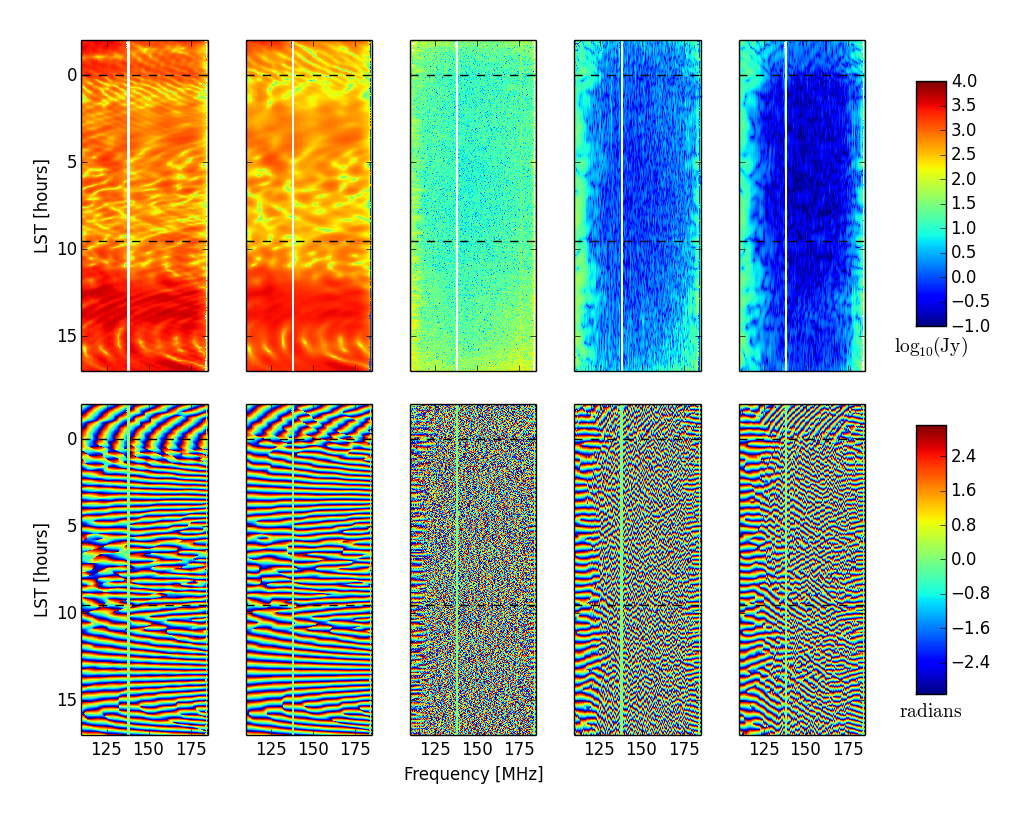
\includegraphics[width=2.3\columnwidth]{plots/waterfalls.png}
\caption{Waterfalls of data.}
\label{fig:waterfalls}
\end{figure*}

For the 30 m East-West baselines used in the power spectrum analysis,
foregrounds are suppressed by $\sim$5 orders of magnitude in power,
effectively getting -50 dB of foreground suppression. The signal loss associated
with this type of filter is the same as in \cite{parsons_et_al2014a} because we
are using same filter with the same 15 ns buffer outside the horizon per
baseline.  We reiterate the results here: there is a 4.8\% signal loss for the
first mode outside of the horizon, 1.3\% for the next mode out, and less than
.0015\% for the higher modes.

After the wideband delay filter, we conduct another round of RFI and crosstalk
removal which was overshadowed by the foreground signal. For RFI excision we
apply a median filter which flags above $3\sigma$. Foregrounds kept us using the
traditional method of removing cross talk which consisted of subtracting hour
long averages from each visibility. This was due to the fact that some days in
the observation had gaps in time owning to some technical difficulties during
observations. However, with foregrounds removed we were able to remove 10 minute
averages from every visibility within a file (files have a cadence of ten
minutes). Normally, hour long averages are needed for foreground contained data
to wash out the fringes from the said foregrounds to detect the static phase
bias that is crosstalk. For foreground removed data, we do not have this
complication since bright foregrounds are not dominating the average and are
able to remove the offset by subtracting shorter sums.


\section{LST Binning and Stability}\label{sec:lstbin}
%   -Practicals: bin size, number of days, range of days 
%       --We LST bin the data over the 120 night data set into time bins of
%         42.95 seconds. 
%       --WE form multiple LST data sets which bin different days throughout the
%       observation together. These datasets help us remove systematics in the
%       power spectrum estimation. They also provide us a way to jackknife the
%       data set.
%   -N lst data sets. Jack-knifing etc.
%   -Median Filter : no signal loss. Filtering because of outliers in time that
%    find their way into the data 
%       --While lst binning, we apply a median filter which for a given lst and
%       frequency bin, removes data which falls outside 3 sigma of the median of
%       the dataset. This filtering is necessary, because of the non gaussian
%       events that crept their way into the data set, such as RFI, etc...
%       --There is no signal loss associated with this because we are using
%       median statistics. 
%   -Plots: Integration counts vs. LST/freq  waterfall.

Once smooth sources have been removed and a final pass of RFI excision and
crosstalk removal have been performed, the data is averaged in local sidereal
time (LST) with bins of width 43 seconds to match the fringe rate filter applied
in the compression. The averaged data set consisted of 135 unevenly sampled
days with the effective number of total days being 123.57. 

Sporadic RFI events can skew individual LST bins away from the median value of
the sky at a given LST, deviating from gaussian statistics. To catch these
events, we compute the median of a LST bin for each frequency and flag off 3
sigma outliers of the median before averaging. This filter mitigates
the effects of non gaussianity in time, which is most likely due to spurious
RFI events. The median statistics used here necessitate that there is no signal
loss due to this filter.

We make two separate lst binned data sets, averaging every other julian day
together to obtain an "even" and "odd" dataset. The use of these two data sets
allows us to conststruct an unbiased power spectrum estimate, as well as running
jackknife tests on our observations. 

One of the key aspects of PAPER is the stability of the instrument between
baselines and in time. Figure \ref{fig:density} shows for a given redundant
group of baselines, the spread in the visibilites for all of the baselines in
that group as a function of LST's. We get more samples per LST bin during the
lst range of 2-10 hours due to our observing season. For each LST bin, the
spread in the samples is ~100 Jy.

\begin{figure*}[!t]
\centering
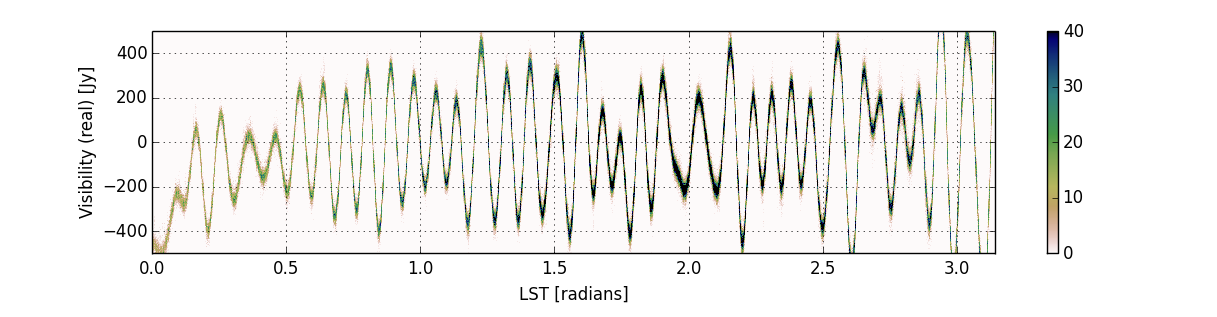
\includegraphics[width=2.3\columnwidth]{plots/density.png}
\caption{Visibility density for a redundant baseline group.}
\label{fig:density}
\end{figure*}

%XXX need to refresh my memort of this plot. FFt of a single baseline, lstbined?
Figure \ref{fig:stability} shows the stability of the instrument as a function
of time. 


\begin{figure}[!t]
\centering
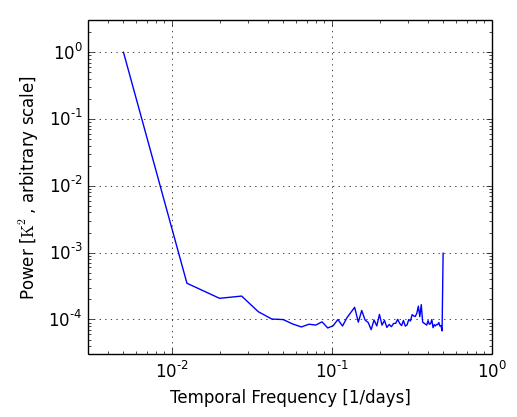
\includegraphics[width=\columnwidth]{plots/stability.png}
\caption{Time stability of the instrument.}
\label{fig:stability}
\end{figure}






%\subsubsection{A noise study}
%During the LST averaging, we compute the median and the variance for every LST
%and frequency bin. The variance in particular is of importance becuase it allows
%us to estimate the system temperature, $T_{sys}$, as a function of LST and
%frequency. The variance is computed, per frequency, for all the visibilities
%that are included in a given LST bin, which gives us an estimate ${I_{rms}}$,
%the specific intensity in Jy, which is then converted to a $T_{rms}$ in the
%usual way, 
%\begin{equation}
%    T_{rms} = \frac{I_{rms}\lambda^{2}}{2k\Omega}.
%\end{equation}
%
%where $\lambda$ is the observing wavelength, $\Omega$ is the size of the beam in
%steradian, and $k$ is the boltzmann constant. We convert $T_{rms}$ to a system
%temperature by scaling up the rms with the effective integration time and
%bandwidth used. That is, 
%\begin{equation}
%    T_{sys} = T_{rms} \times \sqrt{\Delta{B}t_{int}}.
%\end{equation}
%
%Figure \ref{fig:tsys_lst_fq} shows the system temperature as a function of
%LST and frequncy. In our "cold" patch, we find that $T_{sys}$ is around $500K$.
%
%
%\begin{figure}
%\centering
%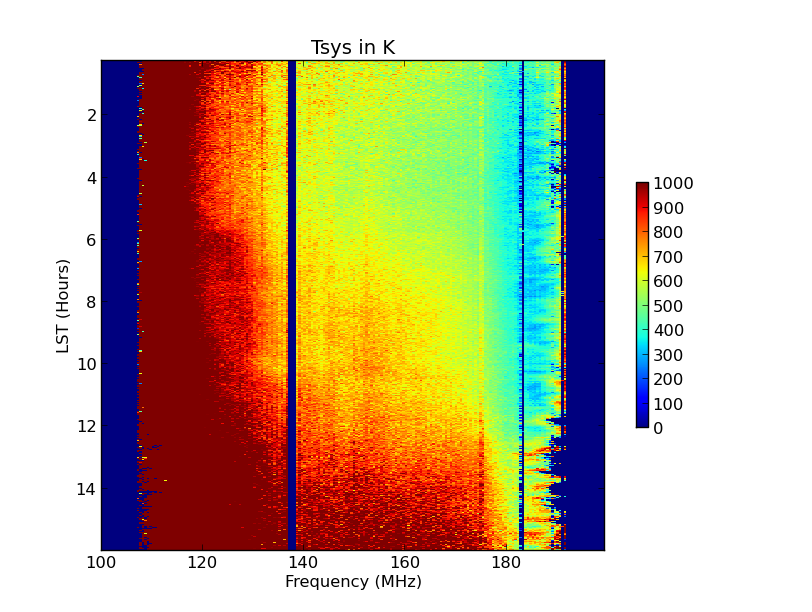
\includegraphics[width=\columnwidth]{plots/tsys_lst_freq.png}
%\caption{Tsys as a function of lst and frequency. The cold spot resides in the
%lst range of 1-7hours.}
%\ref{fig:tsys_lst_fq}
%\end{figure}






\subsection{Optimal Fringe-Rate Filter}\label{sec:frf}
%   -What is fringe rate filtering. Cite Parsons And Liu 2014.
%       --Fringe Rate filtering is nothing more then a time domain weighted
%         average per frequency of of visibilities. The filter can be applied 
%         as either a convolution in the time domain or a multiplicative fourier
%         filter in fringe rate space. 
%       --We first calculate fringe rate filter such that we upweight the more
%         sensitive fringe rates versus the not so sensitve fringe rates by
%         weighting the fringe rates for a given baseline by its beam.
%   -Effective beam areas.
%       --When fringe rate filtering, we are upweighting fringe rates that
%         are most sensitive. That is we are weighting these fringe rates by the
%         beam of a baseline. This has the effect of narrowing the effective
%         beam. It turns out that we are removing more noise than signal,
%         because we are essentially keeping the most sensitive parts of the
%         sky. This actually gives us a sensitivity boost of about a factor of
%         2. 
%   -effective integration time and number of modes. 
%       --Do calculations.
%       --Fringe rate filtering is effectively a weighted average in time and
%       thus there is an effective integration time. We can calculate this
%       integration time by noting that power (or variance) is a conserved
%       quantity. Therefore, comparing the integral of a variance=1 noise signal
%       when it is fringe rate filtered to when it is not, gives us a fractional
%       integration time. 
%           \frac{ \int_{t_{start}}^t_{end}{\sigma^{2}*F_{constant}(t)dt
%           }}{\int_{t_{start}}^t_{end}{\sigma^{2}*F_{filter}(t)dt = fraction.
%            t_int = fraction * t_start-t_end
%           Something like that.
%       --Due to the fact that fringe rate filtering is effectively averaging in
%         time, A fringe rate filter reduces the number of independent modes on
%         the sky. The number of modes in an entire day drop just 45
%         (24hrs/1900sec)  independent modes on the sky. 
%   -PLOTS: 
%       --FR filter (both in fr and time space), applied to data.
%       --Beam after fringe-rate filter. 
%       --Waterfalls.
%       -- apply filters to foreground data. Compute fr of pica and show that we
%          are not killing the sky.
%   
%   code to get the integration time of fringe rate filter. This is 1886 for channel 100
%   beam_w_fr = frf_conv.get_beam_w_fr(aa, (1,4))
%   t,firs,frbins,frspace = frf_conv.get_fringe_rate_kernels(beam_w_fr, 42.8, 401)
%   fr100 = frspace[100]
%   t_int = 42.8/n.mean(fr100)
%   

Prior to forming power spectra we need to time average visibilities that measure
the same $k$ mode on the sky. The motivation for this is that we want to combine
coherent $k$-modes on the sky before squaring to get the maximum sensitivity. We
therefore get a $\frac{1}{N}$ sensitivity boost, rather than averaging in $P(k)$
which would only give us a $\sqrt{N}$ sensitivity benefit. However, rather than
a straight average, we can apply a carefully crafted fringe-rate filter that
weights higher sensitivity portions of the sky higher than those lower in the
sky.

Broadly, for a given baseline and frequency, different parts of the sky
correspond to different fringe-rates, albeit not a one-to-one correspondense.
Maximum fringe rates are found along the equatorial plane, where the rotation
rate of the earth is highest, and zero fringe rates are found at the poles,
where the rotation rate of the earth is zero and hence sources do not move
through your baelines fringe pattern. We can use this fact to pick out certain
points on the sky, but because this mapping of fringe-rate to sky is not one to
one, we can only pick out stripes of constant fringe rate.

As motivation, we discuss the use of fringe rate filters in cross talk removal.
Crosstalk is modeled as a time independent coupling of signal between two
different signal paths, be it at the antenna or to to input our the analog to
digital converters. Since crosstalk does not vary as a function of time, in
fringe rate space, cross talk piles up at the poles which correspond to zero
fringe rates. In this view crosstalk is a DC bias. To remove crosstalk, we can
apply a notch filter to the fringe rate transform of the time series visibility
(per frequency) and inverse transform to go back into time domain. This
interpretation of crosstalk being a DC offset jives with our method of crosstalk
removal discussed above. In order to remove a DC offset from a time series, we
subtract the average.

Now, to optimally combine the time data we can cater our fringe rate filter to
upweight points of the sky that contain more signal to our instrument and down
weight those points that do not. That is, if we weight fringe rate
bins by the beam, we can get a net increase in sensitivity. Roughly, all fringe
rate bins contain the same amount of noise in them, but the amount of signal
varies and is determined by how the primary beam illuminates the sky.
Upweighting the bins with higher signal relative to those with less signal
gives us a net increase in signal-to-noise, even though we are removing 
signal by applying signal from this filter. 

The effective beam area from applying an optimal fringe rate filter decreases,
which implies that the signal has been attenuated, as noted above. But because
the noise is attenuated more, because of beam weigting fringe rate bins, the SNR
increases. For the PAPER array, the boost in SNR is a factor of 2. The net boost
in SNR depends on where the array is located. 

We implement the optimal fringe rate filter by calculating the fringe rates at
every point on the sky, for a given frequency, and weighting each bin by the
beam of a given baseline. It is worth noting that fringe-rate filtering is
baseline dependent and hence is implemented on a per baseline basis. We weight
the fringe rate bins on the sky by the beam pattern at the same point on the
sky. In order to obtain a smoothe filter in the fringe rate domain, we fit a
gaussian with a tanh tail to this filter as shown in figure
\ref{fig:fringe_rate_cut}. We then fourier transform this to obtain the time
domain filter, multiply by a blackman-harris window function to damp the tails
of the filter, and finally convolve with the visibilites to effect time domain
integration.

Since the PAPER beam is ~45 degrees, and the array is located at a declination
of $-30^{\circ}$ the fringe rates associated with the low signal to noise (down
in the beam) correspond to very high and very low/negative fringe rates. Figure
\ref{fig:fringe_rate_cut} shows a cut of the optimal fringe rate at 159 MHz for
a 30 m east west baseline. Therefore, the implemented fringe rate filter removes
some sky signal, signal associated with fringe rates outside of the ranges shown
in Figure \ref{fig:fringe_rate_cut}. Figure \ref{fig:fr_preserved_signal} shows
that the applied filter removes sky associated with negative fringe rates and
very high fringe rates. 

\begin{figure}[!t]
\centering
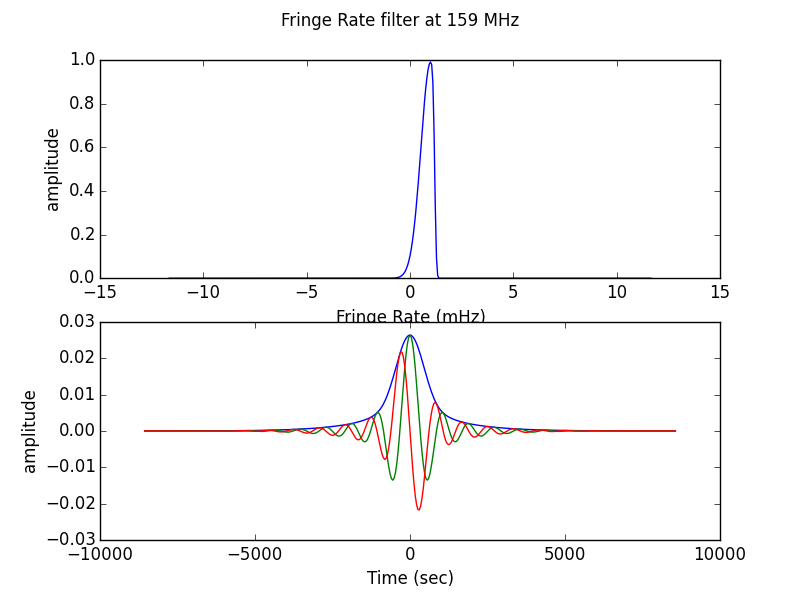
\includegraphics[width=\columnwidth]{plots/fr_filter_slice.png}
\caption{slice of a fringe rate filter at a frequency of 159MHz. Top is the
filter in fringe rate domain. The bottom consists of the corresponding time
domain filter gotten by fourier transforming and windowing with a
blackman-harris window to damp the tails.}
\label{fig:fringe_rate_cut}
\end{figure}

\begin{figure*}[t!]\centering
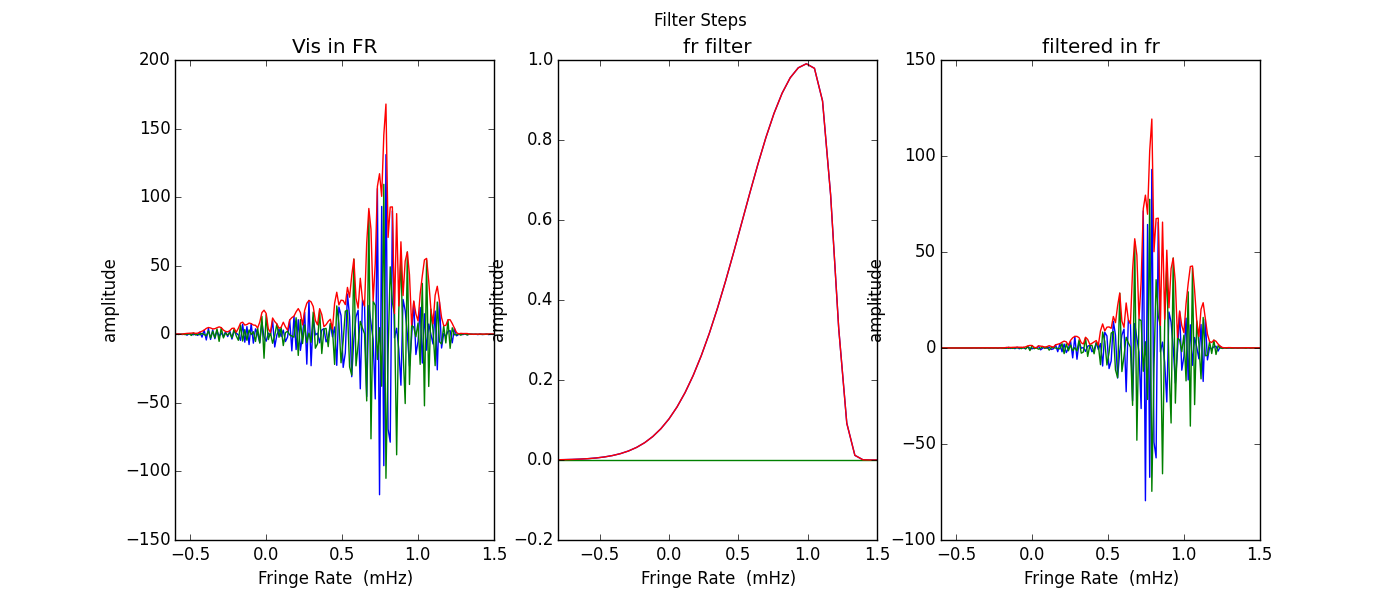
\includegraphics[width=2\columnwidth]{plots/fr_preserved_signal.png}
\caption{slice of a fringe rate filter at a frequency of 159MHz. Shown here is
the fringe-rate transform of foreground contained data for a 30 m east-west
baseline. Blue and green are the real and imaginary part, respectively and red
is the absolute valeu. Note the maximum and minimum fringerates correspond to
the theoretical minimum and maximum for a baseline of this length at 159 MHz.
The center panel shows the real (red)  and imaginary (green) parts of the fringe
rate filter to be applied. Finally, the last panel on the right shows that the
fringe rate filtered visibilities. The fringe rate filter is just a weighting
applied in fringe rate space and retains foregrounds.}
\label{fig:fr_preserved_signal}
\end{figure*}

For the power spectrum baselines in question (30 m East-West baselines), the
effective integration time is calculated by comparing the variance statistic for
a fringe rate filter that is a flat weighting vs that with an optimal filter
weighting as described. We apply these filters to random noise with variance 1,
without loss of generality. We can conclde that 
\begin{align}
    t_{int} &= \frac{\int{\sigma^{2}dt}}{\int{\sigma^{2}fr^{2}dt}}\\
            &= 1886 \text{seconds},
\end{align}
for an optimal fringe rate filter on a 30 m East-West baseline at 149.5 MHz.
Over the range of frequencies used in our power spectrum estimate, the
integration times range from 1936 s to 1790 s, correspinding to an average of 31
minutes. Because the fringe rate filter in effect integrates in time, the number
of statistically independent samples of the sky drastically decreases. We are
left with $\sim2$ independent samples per hour.

%\begin{figure}[h!]\centering
%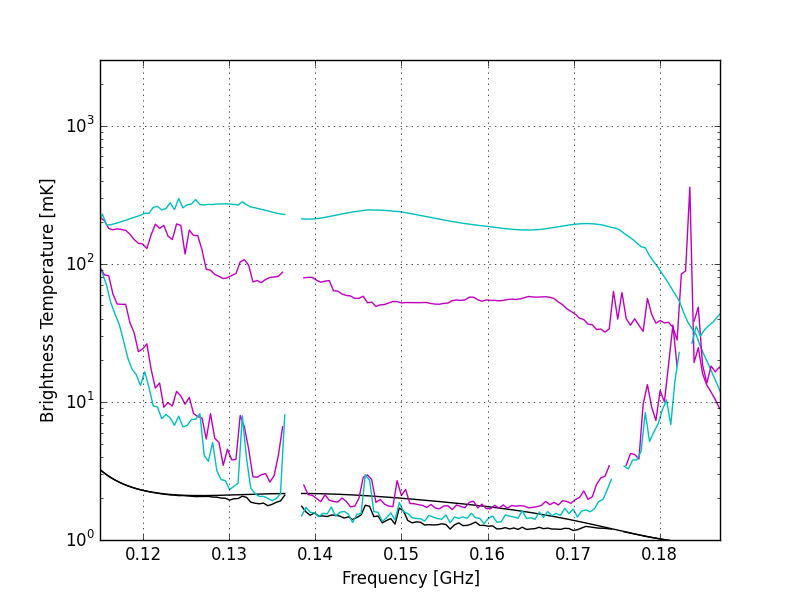
\includegraphics[width=\columnwidth, height=.8\columnwidth]{plots/noise_t_35.png}
%\caption{Estimates of noise temperature. Magenta is frequncy differenced
%estimate where the cyan is the time differenced estimate. All curves are
%averaged over all 30m east-west baselines (56) and averaged incoherently in 43s
%bins of LST from LST 3 to 5 hours with a channel bandwidth of 490 kHz.}
%\label{fig:noise_t}
%\end{figure}


%\begin{figure}[h!]\centering
%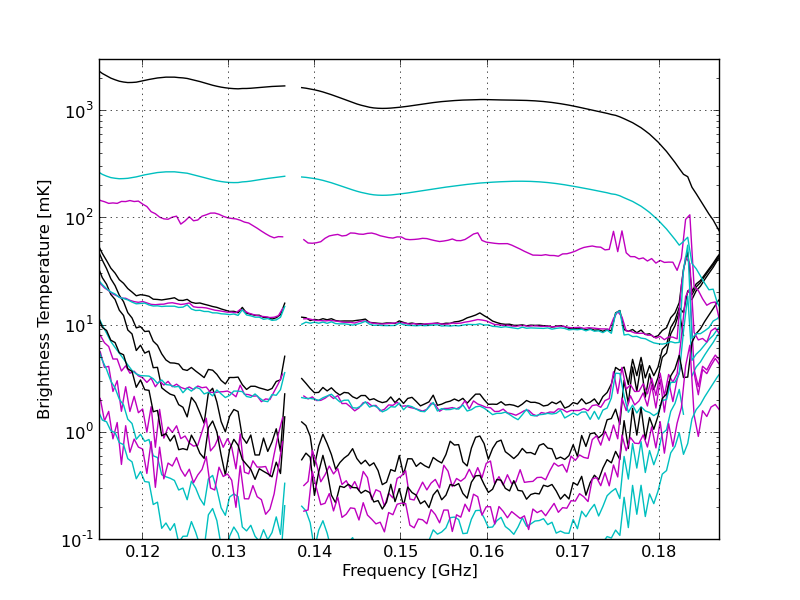
\includegraphics[width=\columnwidth, height=.8\columnwidth]{plots/noise_vs_fq_plot.png}
%\caption{Estimates of noise temperature. Magenta is frequncy differenced
%estimate where the cyan is the time differenced estimate. Averaged in LST from 3
%to 5 hours. on uv files calibrated with omnical. fg,delay filtered, baseline
%averaged, normal fringe rate filter, optimal fringe rate filtering.}
%\label{fig:noise_omni_uv}
%\end{figure}


\subsection{Optimal Quadratic Estimator and Covariance}\label{sec:oqe}
%   -Motivate method with discussion of empirical estimate of covariances and
%    problem of limited modes.
%       --Because we dont know the true covariances between baselines and
%         channels we have to estimate the covariances epirically from data. 
%       --We do this by taking the outer product of our data vector (consisting
%         of a visibilies for every baseline of a given unique baseline type).
%         The outer product is calculated per time sample, thus we average over
%         a "clean" (what do i mean by this?) lst range.
%       --Hence, the quality of the estimate of the covariances between
%         baselines depends on the average in time ( the ensemble average). 
%       --The fact that we do not know what the full covariance matrix looks
%         like leads to signal loss. We have an estimate of the covariance, not
%         the true covariance matrix. There is no way to truly know what the
%         covariance matrix is for our data set. 
%       --After fringerate filtering, the number of independent modes on the
%         decreases substantially because we are averaging over 1900 seconds
%         ~=31.67 minutes. Therefore the number of independent modes decreases
%         1900/(the beam in time). 
%       --In our range of lsts used, we only have roughly 20 independent
%         samples. Therefore we end up with an ill determined covariance matrix
%         to describe our data. 
%       --In addition, because of the highly redundant nature of the array,
%         the covariance matrix is highly singular and therefore not invertible.
This section is divided to break up the formalism and practical use of the
optimal quadratic estimator method to measure the power spectrum. We first
review the formalism, with an emphasis on our analysis, followed by a walk
through of our application of the OQE method to our data, and finally discuss
the effects of an empirical estimate of covariance matrices.



%
%   -Mathematics compared to ideal optimal Quadratic Estimator.
%       --In the quadratic estimator formalism, the value of the power spectrum,
%         $p_{\alpha}$  in the $\alpha^{th}$ bin is given by
%         $Mq_{\alpha}=$Mx^{\dagger}C{-1}Q_{\alpha}C^{-1}x, where x is a vector
%         containing the binned data in frequency domain, $x = V(\nu)$, C is the
%         estimate of the covariance matrix of of our data, C = <xx^{\dagger}>,
%         $Q_{\alpha}$ is defined such that $Q_{\alpha}=\frac{dC}{d\alpha}$, and
%         M is a normalization matrix that normalizes the estimator.
%       --Generally, the covaraince matrix used is the full covaraince between
%         all baselines and channels. 
%       --Because of redundancy, the matrix is singular and not invertible. We
%         therefore construct a pseudo inverse for C. In addtion to the psaudo
%         inverse we take only the auto-baseline covarainces, masking out the
%         covariances between baselines. This, is invertible. WE can thus apply
%         the inverse of C in the above equation.
%
%   -Counting of independent modes.
%       --Number of independent modes = 2*#of lst hours used in analysis. This
%         is because 1900 seconds ~ 30 minutes.
\subsubsection{Review}
We use the optimal quadratic estimator method to estimate our power spectrum
\cite{dillon_et_al2013a, liu_tegmark2011}.
Here we briefly review the optimal quadratic esitimator (OQE) formalism with an
emphasis on application to our data. The end goal is to make an estimate of
the 21 cm power spectrum, $P(\k)$, defined such that 

\begin{equation}
\label{eqn:pspec_def}
    \expval{\tilde{T}_{b}(\k)\tilde{T}^{*}_{b}(\k^{\prime})} =
            (2\pi)^{3}\delta^{D}(\k - \k^{\prime})P(\k). 
\end{equation}
For a data vector $\x$, the optimal quadratic estimator is given by 
\begin{equation}
\label{eqn:quad_est}
    \hat{q}_{\alpha} = \frac{1}{2}\x^{t}\mathbf{C}^{-1}\mathbf{Q}_{\alpha}\mathbf{C}^{-1}\x - b_{\alpha},
\end{equation}
up to some normalization matrix $\mathbf{M}$. With the normalization matrix, the
estimate of the power spectrum in bin $\alpha$ is given by
\begin{equation}
    \hat{p}_{\alpha} = \mathbf{M}\hat{q}_{\alpha}, 
\end{equation}
where $\hat{p}_{\alpha}$ is the estimate of the power spectrum.
In our analysis, $\x$ is the set of visibilities for the redundant baselines of
a single column east-west spacing for a frequency spanning 10 MHz centered at
151.5 MHz. To first order we estimate our covariance matrix by taking the outer
product of our data vector with itself, $\mathbf{C} = \expval{\x^{t}\x}$,
collapsing over the time axis. We discuss the consequences of the covariance
matrix later in this section.  $\mathbf{Q}$ is defined as the derivative of
$\mathbf{C}$ with respect to $\alpha$ ($\frac{\partial C}{\partial \alpha}$). The
$\mathbf{Q}$ matrix encodes the delay transform to go from frequency domain to
delay domain, where $P(k)$ can be estimated. Finally, $b_{\alpha}$ is the  bias to
the estimate that needs to be subtracted off. In our analysis, we are
constructing an unbiased estimator and therefore ignore this term. 
The normaliztion matrix is defined such that
\begin{equation}
    \mathbf{W} = \mathbf{M}\mathbf{F}, 
\end{equation}
where $\mathbf{F}$ is the Fisher information matrix, given by $F = cov(\hat{q})
= 2tr(C^{-1}Q_{\alpha}C^{-1}Q_{\beta})$ and $\mathbf{W}$ is 
the window function matrix. The window functions measure the degree to which
power from $k$ bins couple into the measurement of the power measured in the
$\alpha$'th bin.

%   -Cholesky Decomposition and window functions.
%       --The optimal window functions (that minimize the vertical error bars of
%       the estimate, are given by the inverse of the Fisher matrix. However,
%       there is a trade off such that this incorporates information from all of
%       the k-modes. 
%       --Some other choices of the window functions are the square root of the
%       fisher matrix or the identity. 
%       --We use the cholesky decomposition of the Fisher Matrix such that we
%       can write F = LL^{\dagger}, where L is a lower triangular matrix. This
%       is possible for any hermitian positive-definite matrix.
%       --We use L for our window functions because for every k-bin, it does not
%       use information from the k-bins below it. And thus there is no mixing of
%       modes lower than it. 
%       --This is particularly important because it doesn't insures that there
%       is no leakage of the modes within the horizon to modes outside of it.         
%
The normalization matrix is the analysts choice, and is the last chance to
weight the measurements in the power spectrum estimates. Picking $\mathbf{M} =
\mathbf{F}^{-1}$, and hence $\mathbf{W} = \mathbf{I}$, minimizes the error bars
in the final power spectrum estimate with the trade off that the estimate of the
power spectrum in the $\alpha$'th bin is coupled with every other band power.
Even though this choice gives us the smallest error bars possible, we opt for a
different choice of window function as follows. We first take the
Cholesky-decompositon of the Fisher matrix such that $\mathbf{F} =
\mathbf{L}\mathbf{L}^{\dagger}$, where $\mathbf{L}$ is a lower triangular
matrix\footnote{This is possible for any positive definite matrix}. Then, we
take ${\mathbf{M}} = (\mathbf{L}^{\dagger})^{-1}$ to be our normalization
matrix. In this case, the window function matrix becomes,
$\mathbf{W}=\mathbf{L}^{\dagger}$. This choice of $\mathbf{M}$ has the effect on
the final estimate of the power spectrum in the $\alpha$'th bin of only coupling
modes exterior to $\alpha$ in to the estimate.  This has the consequence of not
coupling the modes inside to horizon in to measurments of the power spectrum
outside the horizon. Figure \ref{fig:window_func} shows these window
functions.

\begin{figure}[h!]\centering
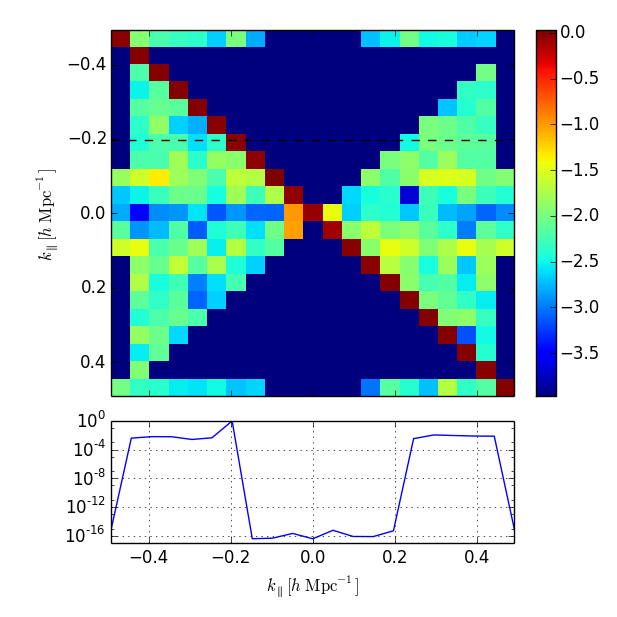
\includegraphics[width=\columnwidth, height=\columnwidth]{plots/window.png}
\caption{Window function matrix. The i'th row corresponds to the window function
used in the estimate of the power spectrum for the i'th $k$-mode.}
\label{fig:window_func}
\end{figure}


\subsubsection{Application}
% A walk through of the application to the data.

We apply the quadratic estimator formalism on a per baseline basis, which leads
to a simplification of the equations in the formalism above. For each
baseline, we empirically estimate the covariance matrix and apply the inverse to
the data itself. Figure \ref{fig:inv_cov} shows the application of the
inverse covariance to both foreground and delay filtered data, in the frequency
domain. Applying the invsere covariance to $\x$ down weights the strongest
eigen modes of $\mathbf{C}$ and upweights the weakest eigen modes. In
comparison, for random white noise, the optimal weighting scheme is inverse
variance weighting, which leads to the smallest error bars. For an infinite
sample of random white noise, the covariance matrix would be diagoanl and
applying the inverse covariance would be identical to inverse variance
weighting. The diagonal of this inverse covariance matrix are the eigenvalues
and correspond to the the eigenmodes. Therefore, the most downweighted modes
correspond to the largest eigenvalues of $\C$, and hence the strongest modes.
Similarily, applying the inverse covariance to the baseline data vector, $\x$,
the strongest modes get down weighted. 

\begin{figure*}[h!]\centering
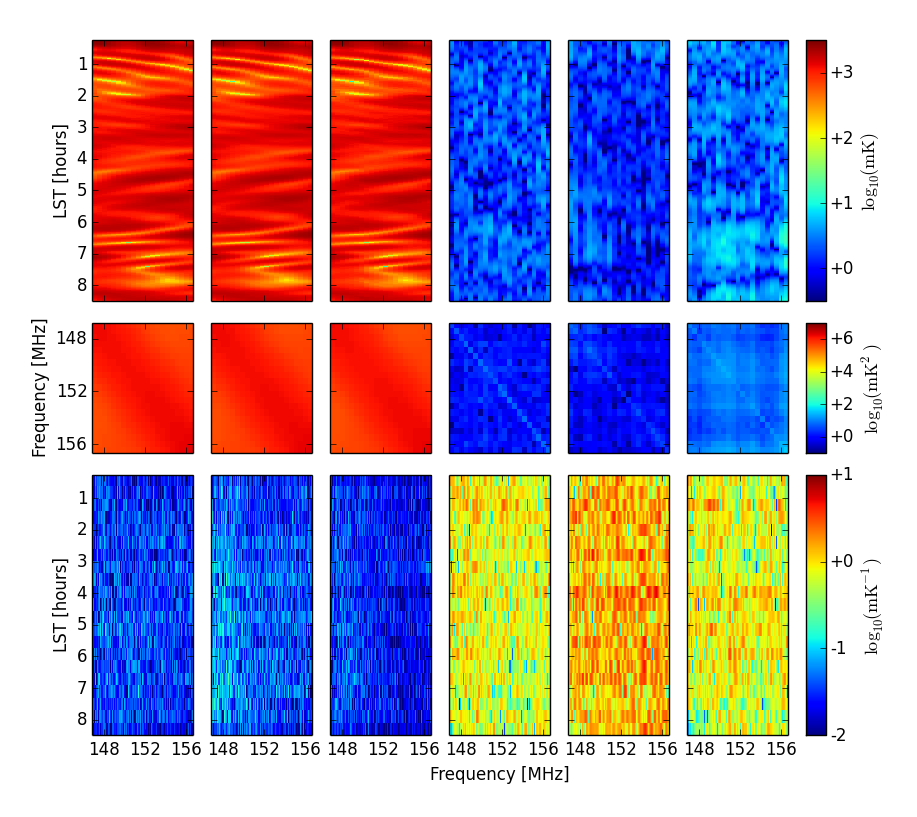
\includegraphics[width=2\columnwidth, height=5.5in]{plots/inv_cov.png}
\caption{Applying the inverse covariance to baseleines.}
\label{fig:inv_cov}
\end{figure*}

For foreground contained data the strongest eigenmodes of the covariance matrix
correspond to delay modes (sine waves in frequency; see figure \ref{fig:eigs}).
In contrast, the strongest modes for delay filtered do not look like clear cut
delay modes, but do have some structure in them. This indicates that there are
modes that describe signal, but are buried in the noise. The strength of these
modes are indicated by eigenvalues of the corresponding covariance matrix. The
strongest eigenmodse for foreground contained to foreground filtered data is
five orders of magnitude, owning to the wideband delay filter.

\begin{figure*}[t!]\centering
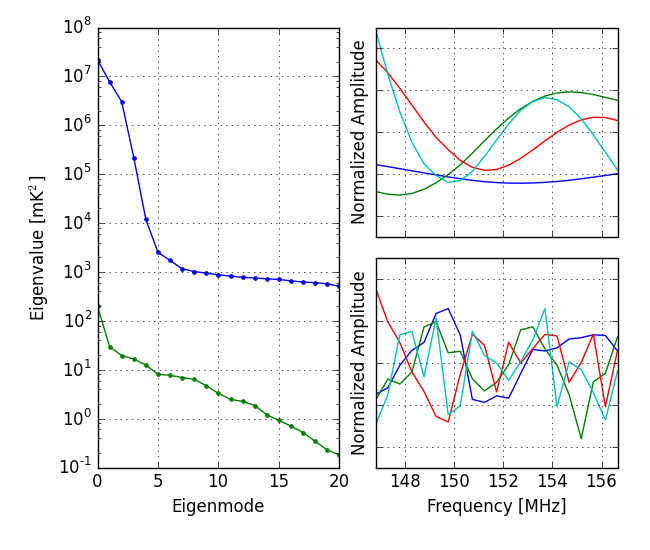
\includegraphics[width=1.5\columnwidth]{plots/eig.png}
\caption{Eigenvalues of the covariance matrix from foreground contained data
(blue) and foreground removed data (green), via the wideband delay filter.
Correspondingly, the strongest four eigenmodes for foreground contained (top
right), and foreground remved data (bottom right).}
\label{fig:eigs}
\end{figure*}

We then construct our optimal estimator by applying equation \ref{eqn:quad_est}
to the baseline data. In the per baseline application, the optimal quadratic
estimator becomes 
\begin{align}\label{eqn:quad_est_perbl}
    \hat{\mathbf{q}}_{\alpha} &=
\sum_{bli,blj}{\frac{1}{2}\x_{bli}^{t}\C^{-1}_{bli}\mathbf{m}_{\alpha}\mathbf{m}_{\alpha}^{t}\C^{-1}_{blj}\x_{blj}}\\
&=
\frac{1}{2}(\sum_{bli}{\x_{bli}^{\dagger}\C_{bli}^{-1}})\mathbf{m}_{\alpha}\mathbf{m}^{\dagger}_{\alpha}(\sum_{blj}{\C_{blj}^{-1}\x_{blj}}),
\end{align}
where $bli$ and $blj$ are 2 different baselines. We neccessarily want to use
baseline cross products in our estimate to avoid incurring a noise bias. The 
$\mathbf{m}$ matrix is half of the $\Q$ matrix in equation \ref{eqn:quad_est},
and encompasses the delay transform. Hence, the two halves of equation
\ref{eqn:quad_est_perbl} are delay transforms.\footnote{This is computationally
beneficial because it requires delay transforming (fft) every baselines data.
This leads to $N_{ch}^{2}\log{N_{ch}} $ computations rather than $N_{ch}^{3}$
computations.} 

Finally, we normalize our power spectrum estimate following the normalization
scheme noted above and choose $\mathbf{M} = \mathbf{L}$, where $\mathbf{L}$ is the lower
diagonal matrix from the Cholesky decompostion of the Fisher information matrix,
$\mathbf{F}$. The Fisher matrix, shown in figure \ref{fig:fisher}, presents the amount
of information there is in every $k_{\parallel}$ mode. The Fisher matrix is
derived using all of the baselines, not just a baseline pair and consists of all
of the information contained in the estimate.
%XXX This part needs work. My understanding of the Fisher Matrix is still
%undeveloped. Noisier modes are upweighted in k-space? 

%Yea...we are not actually doing this. What are we doing?
We apply this method to the sum and difference of the odd and even data sets. We
note that the summed lst data contains signal and noise while the differenced
data set only contains the noise. After computing the power spectrum estimates,
we take the difference of the signal and noise power spectrum to get our final
result. 

\begin{figure}[h!]\centering
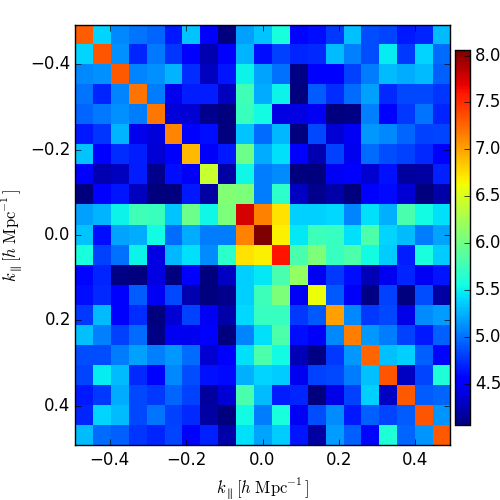
\includegraphics[width=\columnwidth, height=\columnwidth]{plots/fisher.png}
\caption{The Fisher information matrix for a given baseline.}
\label{fig:fisher}
\end{figure}



\subsubsection{The Covariance Matrix}
%Covariance matrix nuances.
%   -describe covariance matrix and data vectors.
%   -How we get the covariance matrix. 
%   -eigenvalue decomposition.
%mode counting and nonsingular-ness.
%   -Count independent modes.
%   -covaraiance is independent only if we have enough indendent modes.
%   -inverse covariance is tricky because of this. 
%   -happy coincidence?
%
%XXX need to check lst range. 

We now discuss the issues of empirically estimating the covariance matrix from
the data. For a single baseline, the data vector $\x$, consists of 10 Mhz
bandwidth centered at 151.72 MHz, equating to 20 frequency channels.
All time samples are also kept, ranging from 0 to 10 LST hours. Again, we
estimate the covariance in the usual way, $\C = \expval{\x\x^{\dagger}}$, taking
the ensemble average over time. The covariance matrix for this baseline is a
$N_{ch}\times N_{ch}$ matrix consisting of the covariances of all channels with
each other. This covariance matrix is invertible only if it nonsingular, which
requires it to be a rank $N_{ch}$ matrix. This occurs only if there are $N_{ch}$
independent modes. 

As noted in section \ref{sec:frf} the optimal fringe rate filter corrsponds to
averageing time samples for 31 minutes. Over the 10 hour LST range used in this
analysis, this corresponds to approximately 20 statistically independent modes
on the sky. This is a fundamental limit of the amount of information we have in
our measurements. Coincidentally, the covariance matrix for a given baseline is
an $N_{ch} \times N_{ch}$ matrix, where $N_{ch}=20$.  Therefore, the covariance
matrices for every baseline are infact invertible because they are full rank 
and contain 20 statistically independent measurements of the sky. The covariance
matrix is thus invertible and can be applied to the data vectors, $\x$. 

%
%   -Potential for signal loss.
%       --In a traditional OQE method, the process is lossless by construction.
%         Because we are tweaking this method, and the fact that we have non
%         gaussian systematics in our data, there is a potential for signal
%         loss. 
Even though we have encountered a fortuitous event in having full rank
covariance matrices, we are still estimating our covariance matrix using a
limited sample size. This limitation leads to an imperfect characterization of
the covariances between modes and ultimately leads to signal loss in this type
of analysis. 

%   -Simulations
%       --In order to show the degree that there could be signal loss, we run
%         simulations to show that an EOR -like signal does pop come out in our
%         data. 
%       --We inject a common eor like signal, a complex random white noise
%         signal, on to all of the baseline data used in this analysisi for a
%         given time. This signal is fringe rate filtered to match the data and
%         therefore, the number of independent modes matches the input data. 
%       --We run this simulation for varying signal levels, showing that this
%         signal can infact be recovered, with some signal loss.
%       --These simulations show that there is signal loss in this method.
%         However, if the signal was bright enough, we would be able to see it.
%         Since we don't see signal in the actual data, we can say that we have
%         not detected the EOR signal yet.

We now characterize this signal loss by running simulations through our power
spectrum pipeline.  In order to understand the degree of signal loss due to our
empirical estimates of the covariances, we simulate the injection of an eor
model and measure the signal loss associated with running the full covariance
analysis. These simulations consist of injecting a model eor signal on top of
the data and running through our power spectrum estimator. In order to
quantify this, we subtract the final power spectrum from one that had no model
injection to measure the final injected signal power spectrum. Comparing this to
the input data gives us an estimate of the signal loss associated with our
pipeline.

%XXX Carina's Text of the eor model goes here.
The model eor signal used was a simulation of a flat power spectrum, in P($k$),
from $k$-modes ranging from .1-10 $\text{hMpc}^{-1}$. From this an angular power
spectrum is computed (\cite{datta_et_al2007, lewis_challinor_2007}), ensuring
correlation in frequency/redshift for the power spectrum maps. Visibilities are
then simulated for this power spectrum map by explicitly integrating fringes on
the sky every 42.8 seconds for an East-West baselin of 30 m.

By using these simulations, we vary the amplitude of the eor signal input into
the oqe by multiplying by a scalar to each simulated visibility. Figure
\ref{fig:simulate} shows that the signal loss is monatonic with increasing
input signal amplitude. With this we argue that if there was an eor signal at
any substatial level, a detection would have been made. Because our power
spectra are still consistent with zero, we conclude that a positive detection of
EoR has not been made. 
%In order to effectively characterize signal loss in our analysis pipeline, we
%simulate visibilities that accurately capture the instrumental effects of PAPER
%for the frequency bins used in the analysis. The signal injected into the
%simulation is comprised of two components - an artificial power spectrum P(k)
%and frequency extrapolated galactic foregrounds from the Global Sky Model (GSM)
%(de Oliveira-Costa et al. 2008). The injected power spectrum is flat in P(k) for
%a k-range of 0.1-10 $\text{hMpc}^{-1}$, and the angular power spectrum is computed from
%this (\cite{datta_et_al2007, lewis_challinor_2007}), ensuring correlation in
%frequency/redshift for the power spectrum maps. PAPER visibilities are simulated
%for both the GSM and power spectrum maps by explicitly integrating fringes on
%the sky every 42.8s for an East-West baseline of 30m.


%Need to argue that the detections are not gaussian and therefore are not eor
%detections.


%   -Maybe : Problem of low noise measurements in this method of analysis i.e.
%    singular matrics - For Adrian.
%
%   -Boot strapping 
%       --In order to calculate the residual noise in our power spectrum
%         estimate, we bootstrap the baseline samples at the output of the
%         quadratic estimator. 
%       --Doing this gives us the variance of the power spectrum estimate and
%         thus derives the 2 sigma error bars shown in the power spectrum. 
%       --We are careful to not incur a noise bias by making sure that the
%         groups used do not contain the same baselines. However, the pull from
%         each group is random with replacement. Each group can have a repeat of
%         a baseline. 
%       --We use 100 bootstraps to derive our error bars, setting a $2\sigma$
%         bound on the errors.

%XXX QUESTION FOR BOOTSTRAPPING, Use the input data to the quad est vs output
%data? Is this why the error bars were so wacked out before?
We measure the error in our final power spectrum estimate by bootstrapping over
baseline samples from the output of the quadratic estimator.
%
%   -PLOTS:
%       --example covariance matrices (with foregrounds, without, fringe rate
%         filtering.
%       --Before and After covariance application waterfall plots.
%
%       --Eigen Spectra and shape of the eigen modes.
%
%       --Window Functions : not waterfalls.
%
%       --Fisher matrices.
%
%       --Power spectrum waterfall plots for different separations. 
%
%       --Maybe the wedge.
%



%\section{Summary of Improvements from PSA32}
%XXX Should this section be here XXX
%In comparison to the previous PAPER pipeline (see \cite{parsons_et_al2014a}),
%this analysis took a slightly different approach which included some critical
%steps to improve our upper limit. In short, the improvements included using a
%new, refined redundant calibration method (Zheng 2014), increasing the width of
%the wideband delay filter that removes smooth spectrum foregrounds, weighting
%the lst binned data sets, and optimal fringe rate filtering. In section
%\ref{sec:analysis}, we dicuss each of the improvements in more detail.
%
%Figure \ref{fig:step_through_pspec} (TBD) shows the power spectra when each of
%the steps mentioned above are turned off and for the one where all of them are
%turned on. We can see the gradual improvement of the power spectra (hopefully).




\section{Results and Discussion}

%   -Tsys, and Tsys vs. time ?


%
%   -Final Pspecs and from various stages 
%       --before/after omnical: Data in
%           /data2/home/zakiali/psa_live/forlstbinning for the before data set.
%           Currently being binned.
%           Note that this data set has ~271 fewer files ~ 48 hours. Hence, it
%           is not the same as the omnical data set.
%           After data set is the one we have always been using : 
%           /data2/home/zakiali/psa_live/forlstbinning_omnical_2 :
%           lstbin_even and lstbin_odd.
%       --before/after frf. Ditto in the above directories.
%       --before after foregrounds. There is foreground data in there as well.
%       SHould we make a foreground run with the non omnical set as well.

%   -Future datasets. Things to look forward to.
%
%   -HERA
%
%   -Relative merrits of foreground avoidance vs fg filtering.
%
%   -relative importance of improvements of psa32.
%
%   -vamp on consistency with zero.
%
%   -Remaining challenges.
%
%       --Polarization leakage.
%       --Sensitivity 
%       --Seeing foregrounds.
%
%
%
%






\subsection{Power Spectrum}
Figure \ref{fig:final_pspec} shows the speherically averaged power spectrum we
measure. Figure \ref{fig:final_posterior} shows the posterior distribution of
the power spectrum by fitting a flat (in $\Delta^{2}$) curve to the
power spectrum assuming gaussian error bars. The posterior distribution uses all
of the data points to determine the 2 sigma upper limit in EoR.
%
%   -Implications for polarized foregrounds.
%       --Flip this around on David and James : We don't see anything at this
%         level, which implies such and such for polarized emission.
%   -Radio recombination and other unsmooth foregrounds. 
%       --paper by peng, Oh. We could maybe confirm this??
%   -Summarize Jonnie's Result.
%   -Repeat the science measurement in Parsons 2014. This will compliment the
%    Jonnies result.
%   -the wedge - maybe?
\begin{figure*}[h!]\centering
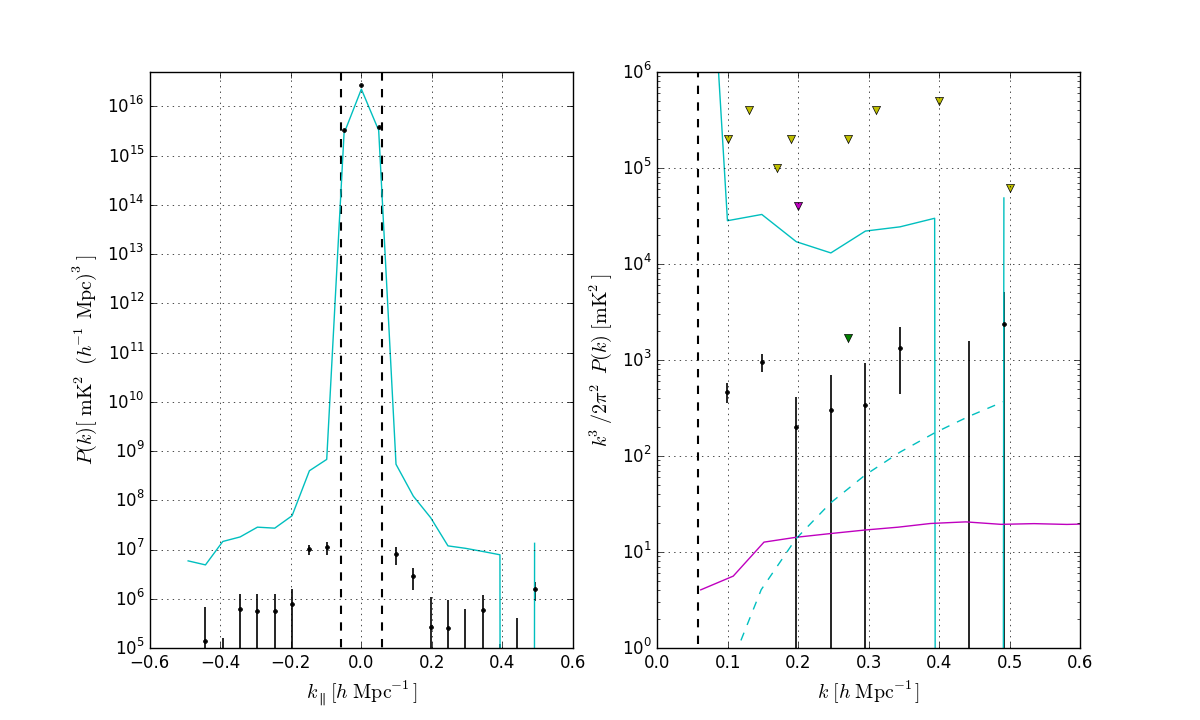
\includegraphics[width=1.5\columnwidth, height=1\columnwidth]{plots/pk_k3pk.png}
\caption{The final power spectrum result.}
\label{fig:final_pspec}
\end{figure*}

\begin{figure}[h!]\centering
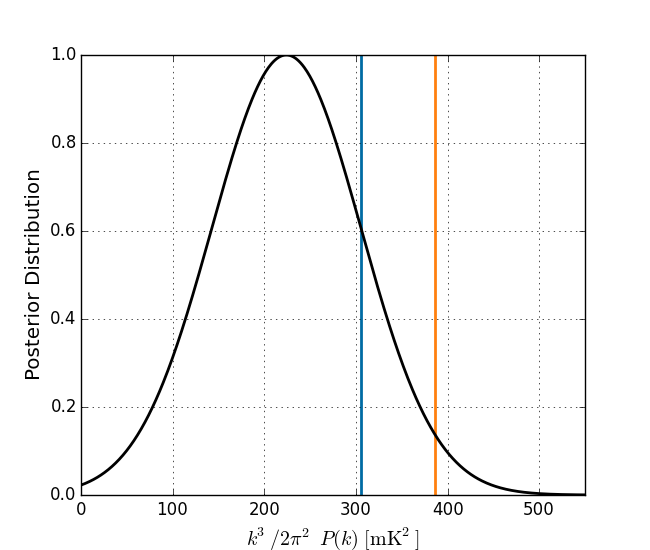
\includegraphics[width=\columnwidth]{plots/flat_k3pk_posterior.png}
\caption{The posteriror distributiom assuming a flat, gaussian spectrum in $\Delta^{2}$.}
\label{fig:final_posterioir}
\end{figure}

\subsection{Noise Levels}   
During the LST binning step, the variance of the visibilities on a frequency and
time basis, are recorded. Using these variance, we calculate the system
temperature as a function of LST, averaging over each LST hour. Figure
\ref{fig:tsys} shows the results of this calculation. In this observing season,
the system temperature decreased significantly, coming down to $T_{sys} = 375K$
at 160 MHz, as compared to \cite{parsons_et_al2014a,jacobs_et_al2014a}, which
used the PAPER 32 antenna data set and deduced a system temperature of 560K at
160 MHz.

\begin{figure}[h!]\centering
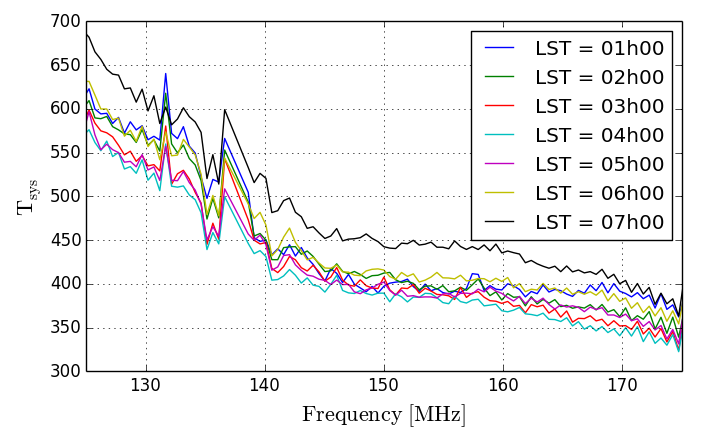
\includegraphics[width=\columnwidth]{plots/tsys.png}
\caption{System temperature as a function of time.}
\label{fig:tsys}
\end{figure}

Offer some thoughts on why this system temperature came down.


\subsection{Comparison with PSA32}
%   -We now compare and contrast our result with those without some of the key
%   components of our analysis pipeline.
%
%   -First we consider the effect from omnical. 
%       -Applying a more precise calibration scheme increases the redundancy
%       between baselines. Hence, this decrease the noise in the measurement. 
%       -This is exactly what we see in the  final power spectrum measurement. 
%       figure \pspecfigure shows the power spectrum of data that has not had
%       omnical applied to it. THe error bars here are reduced by a factor of a
%       few. 
%
%   -Next we consider the effect of using an optimal fringe rate filter. 
%       -By applying an optimal fringe rate filter, we down weight fringe rate
%       bins that are less sensitive, and hence have less signal, and upweight
%       the more sensitive parts of the sky. 
%       -Figure \ref{fig:frf_pspec} shows the power spectrum with a naive fringe
%       rate filer, which is a flat filter and throws out the the fringe rates
%       outside of those possible for a baseline of the eor baselines used in
%       this analysis. 
%       -This gives us a sensitivity benefit of a factor of 3(XXX), as seen
%       in the figure. Note that this data does have omnical applied to it.
%

Here, we discuss the effect to the power spectrum if various stages of the
analysis were kept out. Specifically, we will discuss the effects of using
Omnical and optimal fringe rate filtering vs. not using them. This will give a
sense of how different analyses effect the power spectrum.

The merits of using omnical were described above and it has the effect of
bringing redundant baselines into better agreement with one another by
calibrating out the differences between them. With this picture, we expect
that for the power spectrum, error bars should become tighter. That is the
noise in the measurement would be reduced. Comparing P($k$) for data that has
been Omnical calibrated vs data that has not, but does have the redundant
calibration that was used in \cite{parsons_et_al2014a} applied to it, we see that
the error bars have decreased. This is shown in figure \ref{fig:pspec_nomni}.
Note that the error bars shrink for the higher $k$-modes, the error bars for the
2 modes outside of the horizon do not have this systematic reduction because of
the wideband delay filter. The wideband delay filter is applied after the
calibration solutions have been applied to the visibilities and the 2 modes
outside of the horizon are artifacts of the foregrounds leaking outside of the
horizon. 

\begin{figure}[t!]\centering
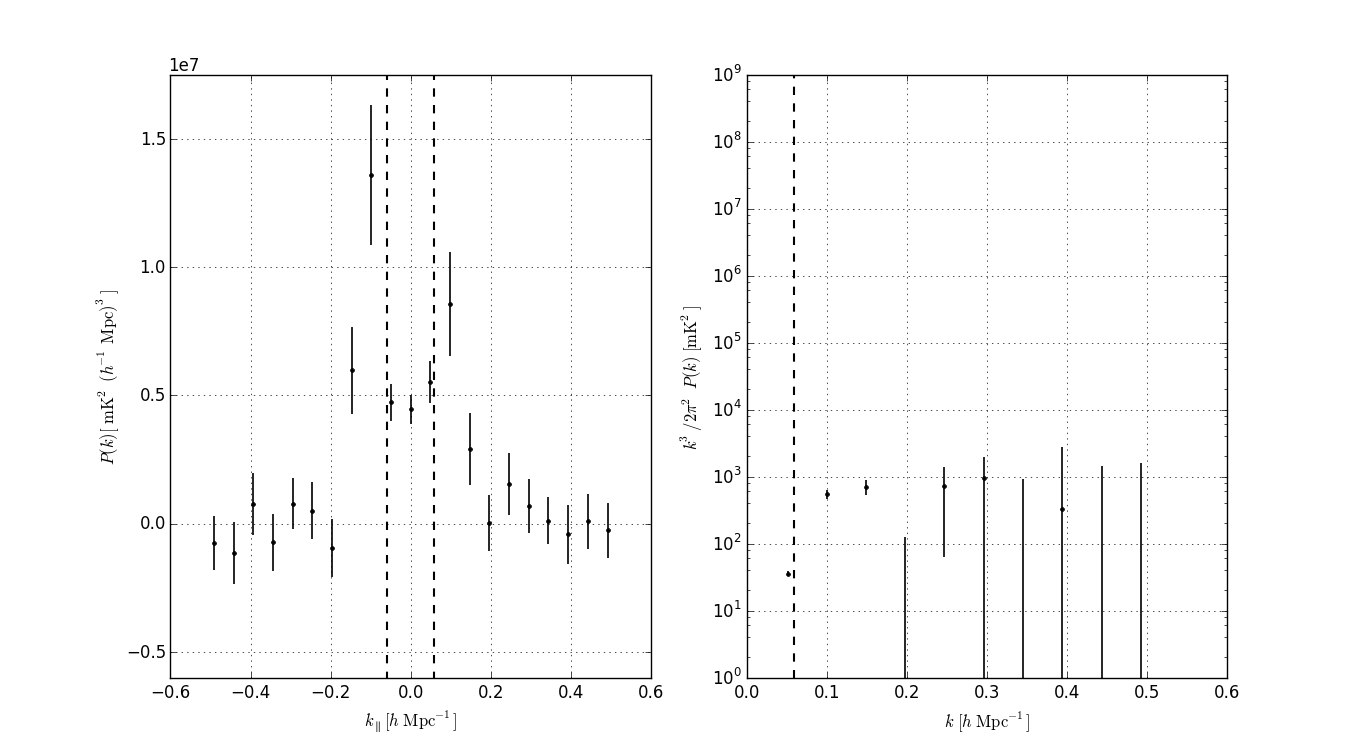
\includegraphics[width=\columnwidth]{plots/pk_k3pk_nomni.png}
\caption{Power spectrum with no omnical applied. Does have optimal fringe rate
        filtering. This plot should be a side by side comparison with and
        without omnical.}
\label{fig:pspec_nomni}
\end{figure}

Optimal fringe rate filtering is a new technique that we have employed in our
analysis and the effect it has on the power spectrum is crucial, considering it
has a sensitivity benefit of a factor of 2. First of all, this fringe rate
filter improves the SNR by a factor of 2 for PAPER, increasing the total
sensitivity of our measurement. Briefly, the filter does this by up weighting
parts of the sky that are illuminated by the primary beam and down weighting
parts of the sky that contain more noise. This has the effect of de noising the
data. Figure \ref{fig:pspec_nofrf} shows the effect of minimal fringe rate
filtering. The filter applied here is the same as described in
\cite{parsons_et_al2014a}. It evenly weights fringe rates from 0 to $f_{max}$,
where $f_{max}$ is the maximum fringe rate possible for a given baseline and
frequency, discarding negative fringe rates. As can be seen in figure
\ref{pspec:nofrf}, the power spectrum in $\Delta^{2}$ comes down by a factor of
2-3. The two modes outside of the horizon, which are dominated by foregrounds
and are clear detections, also come down. The fact that these come down, implies
that the foregrounds are down in the beam possibly near the horizon. Therefore,
the signal there is attenuated by the use of this fringe rate filter. 

It is interesting that at $k\approx.25$, we get a detection of something that
wasnt there before. Foregrounds? probably low level systematics we are hitting
up against. Going to take some convincing...


\begin{figure}[t!]\centering
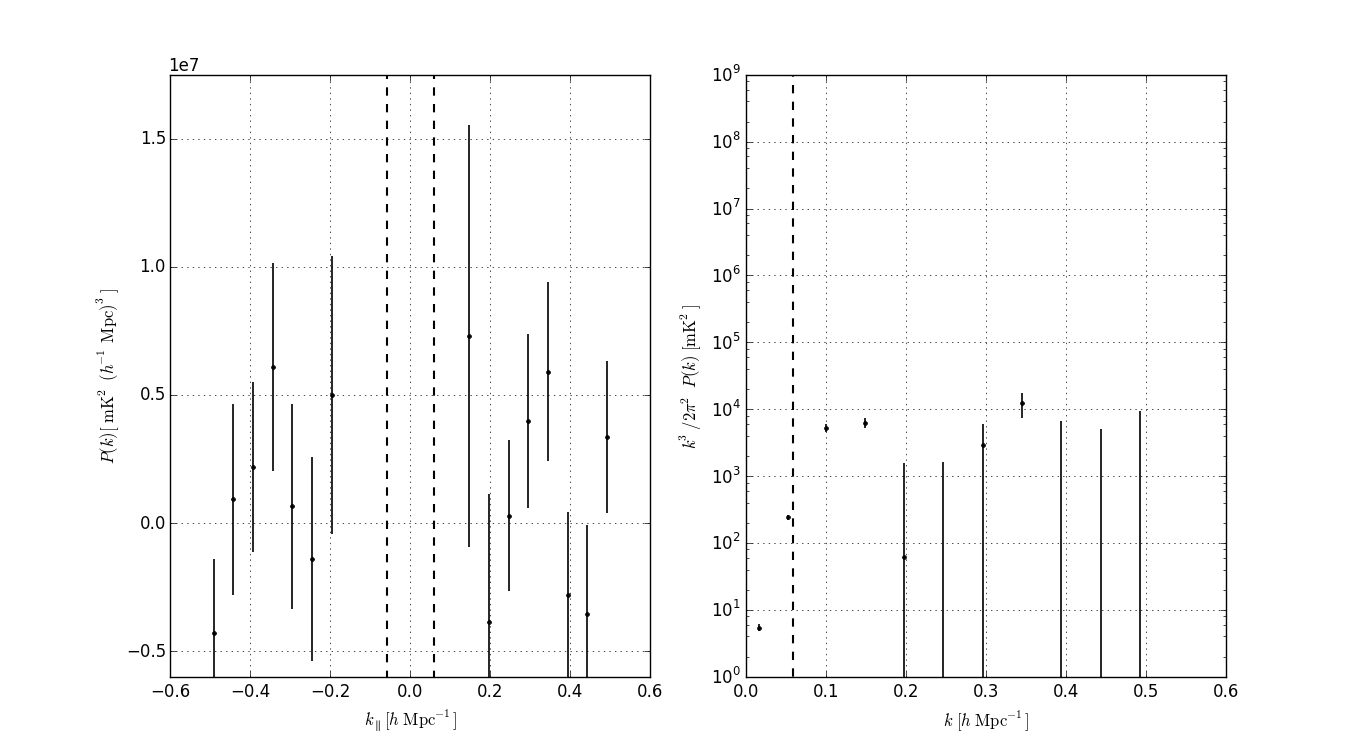
\includegraphics[width=\columnwidth]{plots/pk_k3pk_nofrf.png}
\caption{Power spectrum without optimal fringe rate filtering. Has omnical
applied to it}
\label{fig:pspec_nofrf}
\end{figure}


The new techniques and improvements to calibration used in this analysis are a
considerable improvement from the PAPER-32 analysis from
\cite{parsons_et_al2014a}. These new techniques bring into light the new ways in
which we can gain sensitivity and accurately describe our instrument. The use of
Omnical to accurately calibrate the relative complex gains of the antennas has
shown to be a major improvement to the pipeline. The accuracy and improvement of
this calibration brings redundant baselines more into agreement with one another
and provides and axis for us to check the status of the array. The output 
chi-squared from Omnical provides a metric for us to monitor the health of the
array and another axis for us to flag off bad RFI events. Furthermore, the
precise calbration of antennas is imperative to accurately model and remove
foregrounds. Using the delay spectrum technique employed here, precise
calibration is necessary to mitigate the leakage of foreground power to modes
outside of the horizon for a given baseline. 


\subsection{Future Work}
As the sensitivity of the first generation 21 cm EoR experiments maxes out, the
need for bigger arrays with increased collecting area is necessary. Proposed
experiments such as the Square-Kilometer Array (SKA) and the Hydrogen Epoch of
Reionization Array (HERA) are set to fill this need. HERA is a collaborative
experiment dedicated to detect and characterize the 21 cm EoR power spectrum as
well as eventually image it. The HERA instrument is proposed to be compsed of a
closely packed 547 element array aranged in a hexagon \citep{pober_et_al2014a}.
Each element is a 14-m diamter reflecting-dish, with a total array area of
$\sim.1km^{2}$. Sensitivity forcasts derived in \cite{pober_et_al2014a}
showed that HERA has the ability to make a detection of EoR to a significance
from $\sim32\sigma$ to $\sim133\sigma$ depending on the foreground removal
scheme used. The lower bound is for the delay spectrum technique used in this
paper, where modes within the horizon are irrevocably corrupted, whereas the
higher bound equates to when we can perfectly work within the the wedge. That
is, it is possible to perfectly subtract sources within the horizon.

PAPER itself, is also looking forward to 2 seasons of maximally redundant 128
antenna configuration  data set. This data set has to potential to gain a factor
of $3.5$ in sensitivity as compared to the data set used in this paper. However,
due to constraints on the PAPER site in South Africa, the shortest baselines for
this array are $8\lambda$ (16m), instead of the $16\lambda$ (32m) baselines used
in this analysis. The shorter 8m baselines have not been used in PAPER analysis
before and may be riddled with systematics due to cross coupling and reflections
whithin the array. Therefore, only considering the 16 m East-West baselines,
there will be a total sensitivity benefit of $3$. However, there is the
potential to use the $48m$ nd $64m$ baselines in this analysis as well, boosting
the sensitivity to by another factor of 2.


\subsection{Remaining Challanges}
The closer we get to a detection of the 21 cm EoR fluctuations, the more we need
to know what the systematics can be and at what level they can come in at. One
of the biggest challanges remaining, as metioned above, is the limited
sensitivity of current EoR experiments. Even with the full sensitivity of the
PAPER array at full build out, there will only be a $1.65\sigma$ EoR detection
with the current method of foreground avoidence to detect the power spectrum.
With the complete optimist approach of working withing the wedge, there will be
a $8.86\sigma$ detection of the 21 cm power spectrum \citep{pober_et_al2014a}.
However, the configuration of PAPER makes it difficult to localize sources for
removal and makes it hard to work within the wedge. These sensitivity benefits
are being addressed by second generation EoR experiments, whose goal is to
characterize the 21 cm power spectrum at high redshifts.

In addition to sensitivity limitations, foregrounds are also a challange that
needs to be met. The delay spectrum approach requires that foregrounds need to
be spectrally smooth so that they are localized to inside the horizon. As seen
from equation \ref{eqn:delay_filter}, this approach also requires the need to
know your beam and bandpass very well to mitigate the effect of spreading power
outside the horizon. The PAPER beam is both spaitially and spectrally smooth
\cite{pober_et_al2011}, but even small variations have the effect of
making sppilling power outside of the horizon. In addition to the beam, the
major source of error is in the bandpass. The 9th order polynomial fit to the
bandpass is strictly not just the bandpass but contains ripples imprinted by
sources other than Pictor A. Therefore characterizing the true bandpass of the
instruement is hard and largely unknown for PAPER.

Finally, one of the possibly biggest challenges we face is that of polarization
leakage due to Faraday rotation of polarized sources from Stokes Q into Stokes
I. 

\section{Conclusions}

\section{Acknowledgements}

\clearpage
%\nocite{*}
\bibliographystyle{apj}
\bibliography{biblio}

\end{document}

